\makeatletter
\def\rap@fontpath{../../../Common/}
\makeatother
\documentclass{../../../Common/Latex/Templates/rapport}
% ---------------------------------------------------------------------------
% Shared settings for the H2026 General Assembly document set.
%
% Usage, directly after \documentclass{../../../Common/Latex/Templates/rapport}
% in a document one folder below this file:
%   % ---------------------------------------------------------------------------
% Shared settings for the H2026 General Assembly document set.
%
% Usage, directly after \documentclass{../../../Common/Latex/Templates/rapport}
% in a document one folder below this file:
%   % ---------------------------------------------------------------------------
% Shared settings for the H2026 General Assembly document set.
%
% Usage, directly after \documentclass{../../../Common/Latex/Templates/rapport}
% in a document one folder below this file:
%   \input{../ga-common}
%
% Image paths are relative to the compiled document's folder, so every
% document using this file must sit one folder below it.
% ---------------------------------------------------------------------------

% Meeting details, used on covers and in each document's ID block.
\newcommand{\meetingdate}{30 September 2026}
\newcommand{\meetingtime}{12:00}
\newcommand{\meetinglocation}{Festsalen, NMBU}
\newcommand{\meetingline}{\textbf{Meeting:} \meetingdate, \meetingtime, \meetinglocation}

% Header: moon logo on the left, full-text logo on the right. \projectname is
% still set because the cover title uses it.
\projectname{Eclipse NMBU}
\projectlogo{../../../Common/Eclipse Images/EclipseMoon}
\orglogo{../../../Common/Eclipse Images/EclipseFullText}

%
% Image paths are relative to the compiled document's folder, so every
% document using this file must sit one folder below it.
% ---------------------------------------------------------------------------

% Meeting details, used on covers and in each document's ID block.
\newcommand{\meetingdate}{30 September 2026}
\newcommand{\meetingtime}{12:00}
\newcommand{\meetinglocation}{Festsalen, NMBU}
\newcommand{\meetingline}{\textbf{Meeting:} \meetingdate, \meetingtime, \meetinglocation}

% Header: moon logo on the left, full-text logo on the right. \projectname is
% still set because the cover title uses it.
\projectname{Eclipse NMBU}
\projectlogo{../../../Common/Eclipse Images/EclipseMoon}
\orglogo{../../../Common/Eclipse Images/EclipseFullText}

%
% Image paths are relative to the compiled document's folder, so every
% document using this file must sit one folder below it.
% ---------------------------------------------------------------------------

% Meeting details, used on covers and in each document's ID block.
\newcommand{\meetingdate}{30 September 2026}
\newcommand{\meetingtime}{12:00}
\newcommand{\meetinglocation}{Festsalen, NMBU}
\newcommand{\meetingline}{\textbf{Meeting:} \meetingdate, \meetingtime, \meetinglocation}

% Header: moon logo on the left, full-text logo on the right. \projectname is
% still set because the cover title uses it.
\projectname{Eclipse NMBU}
\projectlogo{../../../Common/Eclipse Images/EclipseMoon}
\orglogo{../../../Common/Eclipse Images/EclipseFullText}

\usepackage{pdfpages}
\usepackage{hyperref}

\reporttitle{Full Document Set}

% ---------------------------------------------------------------------------
% Cover / title page for rapport-class documents.
%
% Usage (after \documentclass{rapport} and before \begin{document}):
%   % ---------------------------------------------------------------------------
% Cover / title page for rapport-class documents.
%
% Usage (after \documentclass{rapport} and before \begin{document}):
%   % ---------------------------------------------------------------------------
% Cover / title page for rapport-class documents.
%
% Usage (after \documentclass{rapport} and before \begin{document}):
%   \input{../cover/rapport-cover}
%   \missionpatch{path/to/patch}      % optional circular mission/team patch;
%                                     % without it, the org logo is shown large
%                                     % at the top instead
%   \coverkind{Vedtekter}             % optional small line above the name
%   \reportsubtitle{Optional subtitle line}
%   \orgname{Eclipse NMBU}{Norwegian University of Life Sciences, Norway}
%   \reportlocation{Ås, Norge}
%   \date{3. oktober 2022}            % optional, defaults to \today
%   \contactinfo{Contact: post@eclipsenmbu.no}  % optional, shown at the bottom
%
% Then, as the first thing inside \begin{document}:
%   \makecoverpage
%
% The large title line shows \projectname (falling back to \reporttitle if
% \coverkind is not set), so a document typically sets both:
%   \projectname{Eclipse NMBU}
%   \coverkind{Vedtekter}
% ---------------------------------------------------------------------------

\makeatletter
\def\@missionpatch{}
\newcommand{\missionpatch}[1]{\def\@missionpatch{#1}}

\def\@coverkind{}
\newcommand{\coverkind}[1]{\def\@coverkind{#1}}

\def\@reportsubtitle{}
\newcommand{\reportsubtitle}[1]{\def\@reportsubtitle{#1}}

\def\@orgnameone{}
\def\@orgnametwo{}
\newcommand{\orgname}[2]{\def\@orgnameone{#1}\def\@orgnametwo{#2}}

\def\@reportlocation{}
\newcommand{\reportlocation}[1]{\def\@reportlocation{#1}}

\def\@contactinfo{}
\newcommand{\contactinfo}[1]{\def\@contactinfo{#1}}

\newcommand{\makecoverpage}{%
  \begingroup
  \thispagestyle{empty}
  \begin{center}
  \ifx\@missionpatch\@empty
    \includegraphics[width=10cm]{\@orglogo}\par
  \else
    \includegraphics[width=6.5cm]{\@missionpatch}\par
  \fi
  \vspace{3.4cm}
  \ifx\@coverkind\@empty
    {\sffamily\Huge\bfseries \@reporttitle \par}
  \else
    {\sffamily\Huge\bfseries \@coverkind \par}
    {\sffamily\Huge\bfseries \@projectname \par}
  \fi
  \ifx\@reportsubtitle\@empty\else
    \vspace{1.6cm}
    {\sffamily\bfseries \@reportsubtitle \par}
  \fi
  \vspace{2cm}
  \ifx\@missionpatch\@empty\else
    \includegraphics[height=1.3cm]{\@orglogo}\par
    \vspace{0.6cm}
  \fi
  \@orgnameone \\
  \@orgnametwo \par
  \vspace{0.6cm}
  \ifx\@reportlocation\@empty
    \@date
  \else
    \@reportlocation, \@date
  \fi
  \par
  \vfill
  \ifx\@contactinfo\@empty\else
    {\small \@contactinfo \par}
  \fi
  \end{center}
  \endgroup
  \newpage
  \pagenumbering{roman}
  \pagestyle{plain}
}
\makeatother

%   \missionpatch{path/to/patch}      % optional circular mission/team patch;
%                                     % without it, the org logo is shown large
%                                     % at the top instead
%   \coverkind{Vedtekter}             % optional small line above the name
%   \reportsubtitle{Optional subtitle line}
%   \orgname{Eclipse NMBU}{Norwegian University of Life Sciences, Norway}
%   \reportlocation{Ås, Norge}
%   \date{3. oktober 2022}            % optional, defaults to \today
%   \contactinfo{Contact: post@eclipsenmbu.no}  % optional, shown at the bottom
%
% Then, as the first thing inside \begin{document}:
%   \makecoverpage
%
% The large title line shows \projectname (falling back to \reporttitle if
% \coverkind is not set), so a document typically sets both:
%   \projectname{Eclipse NMBU}
%   \coverkind{Vedtekter}
% ---------------------------------------------------------------------------

\makeatletter
\def\@missionpatch{}
\newcommand{\missionpatch}[1]{\def\@missionpatch{#1}}

\def\@coverkind{}
\newcommand{\coverkind}[1]{\def\@coverkind{#1}}

\def\@reportsubtitle{}
\newcommand{\reportsubtitle}[1]{\def\@reportsubtitle{#1}}

\def\@orgnameone{}
\def\@orgnametwo{}
\newcommand{\orgname}[2]{\def\@orgnameone{#1}\def\@orgnametwo{#2}}

\def\@reportlocation{}
\newcommand{\reportlocation}[1]{\def\@reportlocation{#1}}

\def\@contactinfo{}
\newcommand{\contactinfo}[1]{\def\@contactinfo{#1}}

\newcommand{\makecoverpage}{%
  \begingroup
  \thispagestyle{empty}
  \begin{center}
  \ifx\@missionpatch\@empty
    \includegraphics[width=10cm]{\@orglogo}\par
  \else
    \includegraphics[width=6.5cm]{\@missionpatch}\par
  \fi
  \vspace{3.4cm}
  \ifx\@coverkind\@empty
    {\sffamily\Huge\bfseries \@reporttitle \par}
  \else
    {\sffamily\Huge\bfseries \@coverkind \par}
    {\sffamily\Huge\bfseries \@projectname \par}
  \fi
  \ifx\@reportsubtitle\@empty\else
    \vspace{1.6cm}
    {\sffamily\bfseries \@reportsubtitle \par}
  \fi
  \vspace{2cm}
  \ifx\@missionpatch\@empty\else
    \includegraphics[height=1.3cm]{\@orglogo}\par
    \vspace{0.6cm}
  \fi
  \@orgnameone \\
  \@orgnametwo \par
  \vspace{0.6cm}
  \ifx\@reportlocation\@empty
    \@date
  \else
    \@reportlocation, \@date
  \fi
  \par
  \vfill
  \ifx\@contactinfo\@empty\else
    {\small \@contactinfo \par}
  \fi
  \end{center}
  \endgroup
  \newpage
  \pagenumbering{roman}
  \pagestyle{plain}
}
\makeatother

%   \missionpatch{path/to/patch}      % optional circular mission/team patch;
%                                     % without it, the org logo is shown large
%                                     % at the top instead
%   \coverkind{Vedtekter}             % optional small line above the name
%   \reportsubtitle{Optional subtitle line}
%   \orgname{Eclipse NMBU}{Norwegian University of Life Sciences, Norway}
%   \reportlocation{Ås, Norge}
%   \date{3. oktober 2022}            % optional, defaults to \today
%   \contactinfo{Contact: post@eclipsenmbu.no}  % optional, shown at the bottom
%
% Then, as the first thing inside \begin{document}:
%   \makecoverpage
%
% The large title line shows \projectname (falling back to \reporttitle if
% \coverkind is not set), so a document typically sets both:
%   \projectname{Eclipse NMBU}
%   \coverkind{Vedtekter}
% ---------------------------------------------------------------------------

\makeatletter
\def\@missionpatch{}
\newcommand{\missionpatch}[1]{\def\@missionpatch{#1}}

\def\@coverkind{}
\newcommand{\coverkind}[1]{\def\@coverkind{#1}}

\def\@reportsubtitle{}
\newcommand{\reportsubtitle}[1]{\def\@reportsubtitle{#1}}

\def\@orgnameone{}
\def\@orgnametwo{}
\newcommand{\orgname}[2]{\def\@orgnameone{#1}\def\@orgnametwo{#2}}

\def\@reportlocation{}
\newcommand{\reportlocation}[1]{\def\@reportlocation{#1}}

\def\@contactinfo{}
\newcommand{\contactinfo}[1]{\def\@contactinfo{#1}}

\newcommand{\makecoverpage}{%
  \begingroup
  \thispagestyle{empty}
  \begin{center}
  \ifx\@missionpatch\@empty
    \includegraphics[width=10cm]{\@orglogo}\par
  \else
    \includegraphics[width=6.5cm]{\@missionpatch}\par
  \fi
  \vspace{3.4cm}
  \ifx\@coverkind\@empty
    {\sffamily\Huge\bfseries \@reporttitle \par}
  \else
    {\sffamily\Huge\bfseries \@coverkind \par}
    {\sffamily\Huge\bfseries \@projectname \par}
  \fi
  \ifx\@reportsubtitle\@empty\else
    \vspace{1.6cm}
    {\sffamily\bfseries \@reportsubtitle \par}
  \fi
  \vspace{2cm}
  \ifx\@missionpatch\@empty\else
    \includegraphics[height=1.3cm]{\@orglogo}\par
    \vspace{0.6cm}
  \fi
  \@orgnameone \\
  \@orgnametwo \par
  \vspace{0.6cm}
  \ifx\@reportlocation\@empty
    \@date
  \else
    \@reportlocation, \@date
  \fi
  \par
  \vfill
  \ifx\@contactinfo\@empty\else
    {\small \@contactinfo \par}
  \fi
  \end{center}
  \endgroup
  \newpage
  \pagenumbering{roman}
  \pagestyle{plain}
}
\makeatother

\coverkind{Full Combined Edition}
\reportsubtitle{General Assembly -- 26H-ECL-GA-FULL1}
\orgname{Eclipse NMBU}{Norwegian University of Life Sciences, Norway}
\reportlocation{\meetinglocation, Ås}
\date{\meetingdate, \meetingtime}
\contactinfo{Contact: post@eclipsenmbu.no}

\includepdfset{pagecommand=\thispagestyle{empty}}

\begin{document}

\makecoverpage
\reportmainmatter

\noindent\textbf{Document ID:} 26H-ECL-GA-FULL1\\
\meetingline\\
\textbf{Purpose:} every document in the General Assembly document set, bound together in one printable edition, in the order given in the Overview (26H-ECL-GA-OVW1). Each document keeps its own Document ID, cover and pagination; this edition adds no new content of its own beyond this page and the blank pages at the end.\\
\textbf{Binding:} this edition is padded with blank pages so its total page count is a multiple of 8, for book-binding in 8-page signatures.

\vfill
\textbf{Contents, in order:} Overview; Notice of Meeting; Agenda; Case Template; Amendment Submission Procedure; Full Meeting Procedure; Timetable and Directions; ID and Abbreviations Reference; Cases 1--4; the Bylaw Amendment (proposed text, plain-language explanation, voting procedure, and the Norwegian originals of both the Old and New Bylaws); C-suite structure; Election of Board Members; Candidate Documentation; Election Ballots; Voting Order; Meeting Protocol; Membership Contract; Responsibility and Signature Contract and Board Record; GF for Dummies; the Glossary. See the Overview (26H-ECL-GA-OVW1) for the exact Document ID of each.

\clearpage


\includepdf[pages=-]{../00 Overview/26H-ECL-GA-OVW1.pdf}

\includepdf[pages=-]{../01 Notice of Meeting/26H-ECL-GA-NOT1.pdf}

\includepdf[pages=-]{../02 Agenda/26H-ECL-GA-AGD1.pdf}
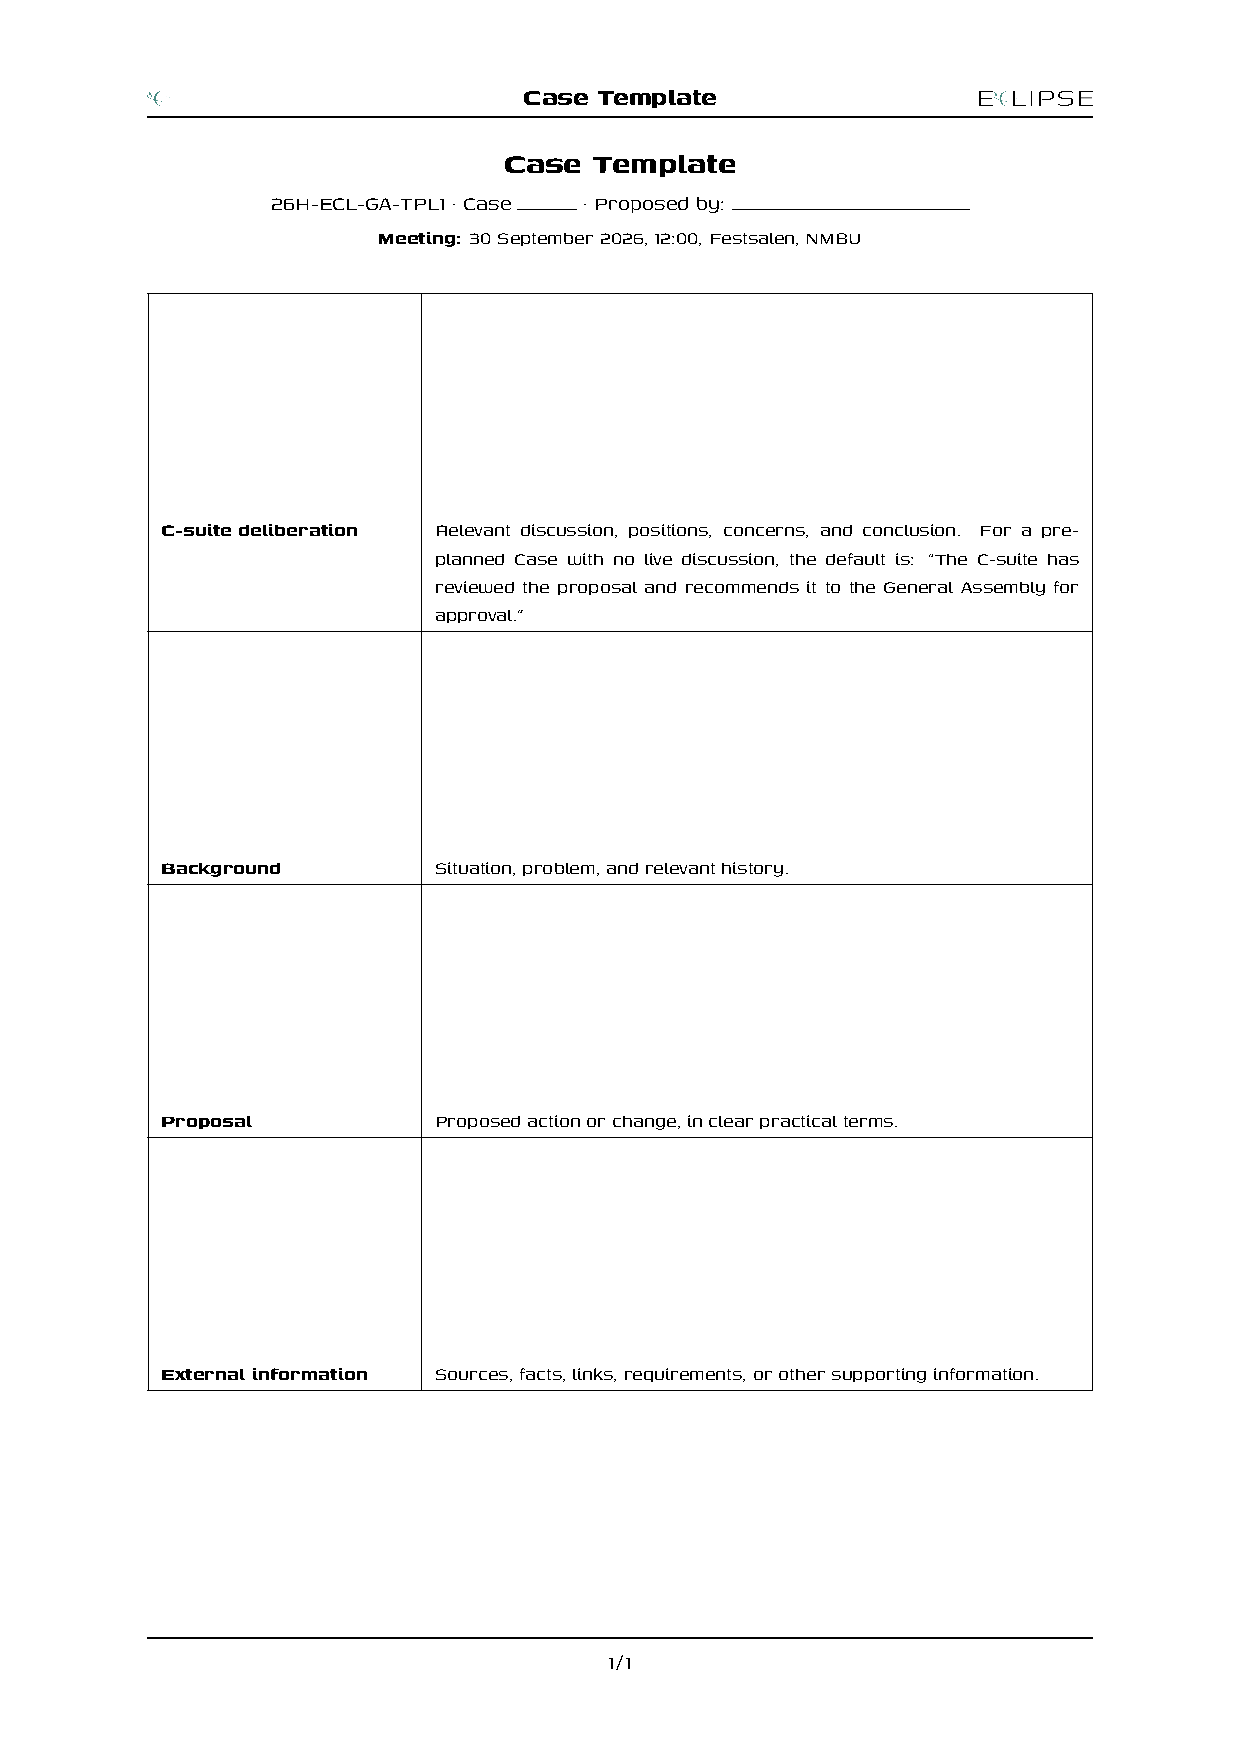
\includepdf[pages=-]{../03 Case Template/26H-ECL-GA-TPL1.pdf}
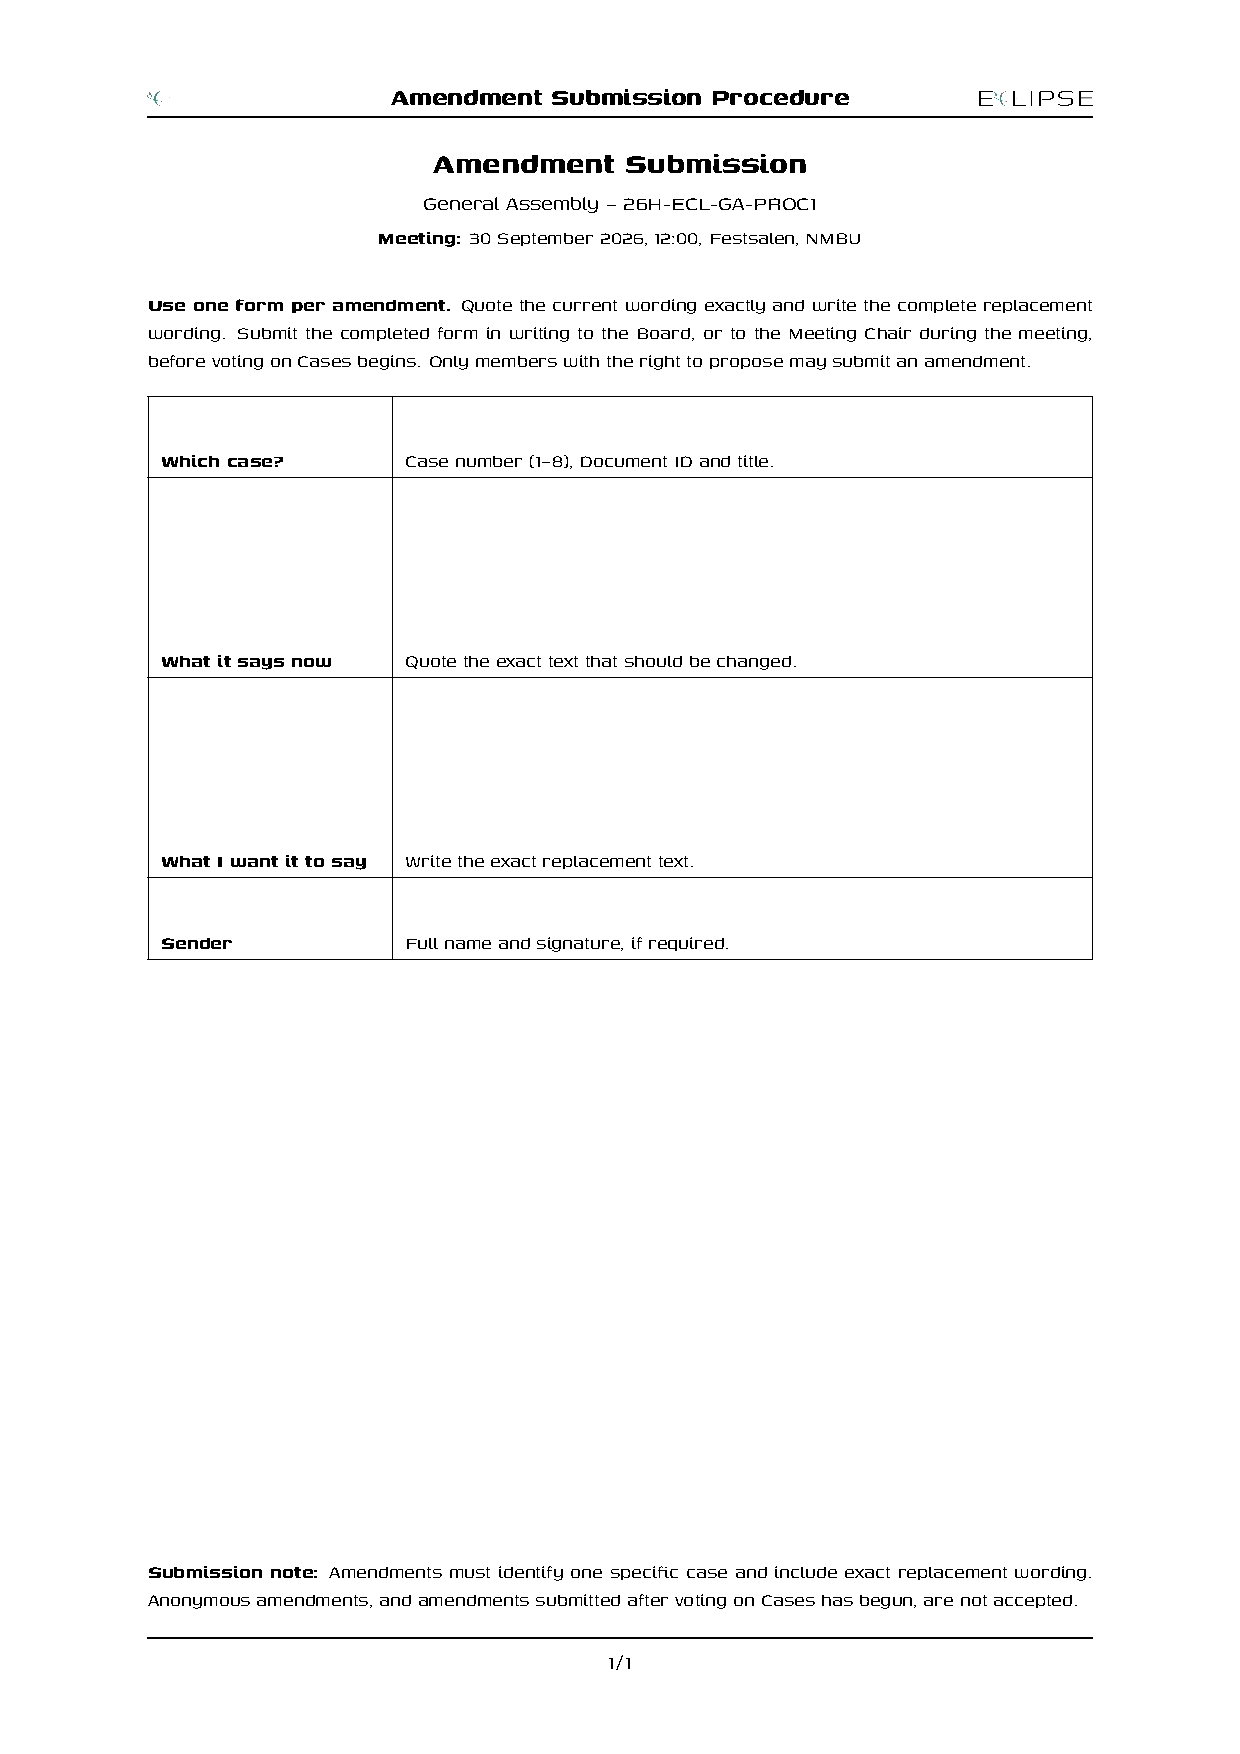
\includepdf[pages=-]{../04 Amendment Submission Procedure/26H-ECL-GA-PROC1.pdf}

\includepdf[pages=-]{../17 Full Procedure (Old Bylaws)/26H-ECL-GA-PROC2.pdf}

\includepdf[pages=-]{../18 Timetable and Directions/26H-ECL-GA-TIME1.pdf}

\includepdf[pages=-]{../19 ID and Abbreviations Reference/26H-ECL-GA-REF1.pdf}
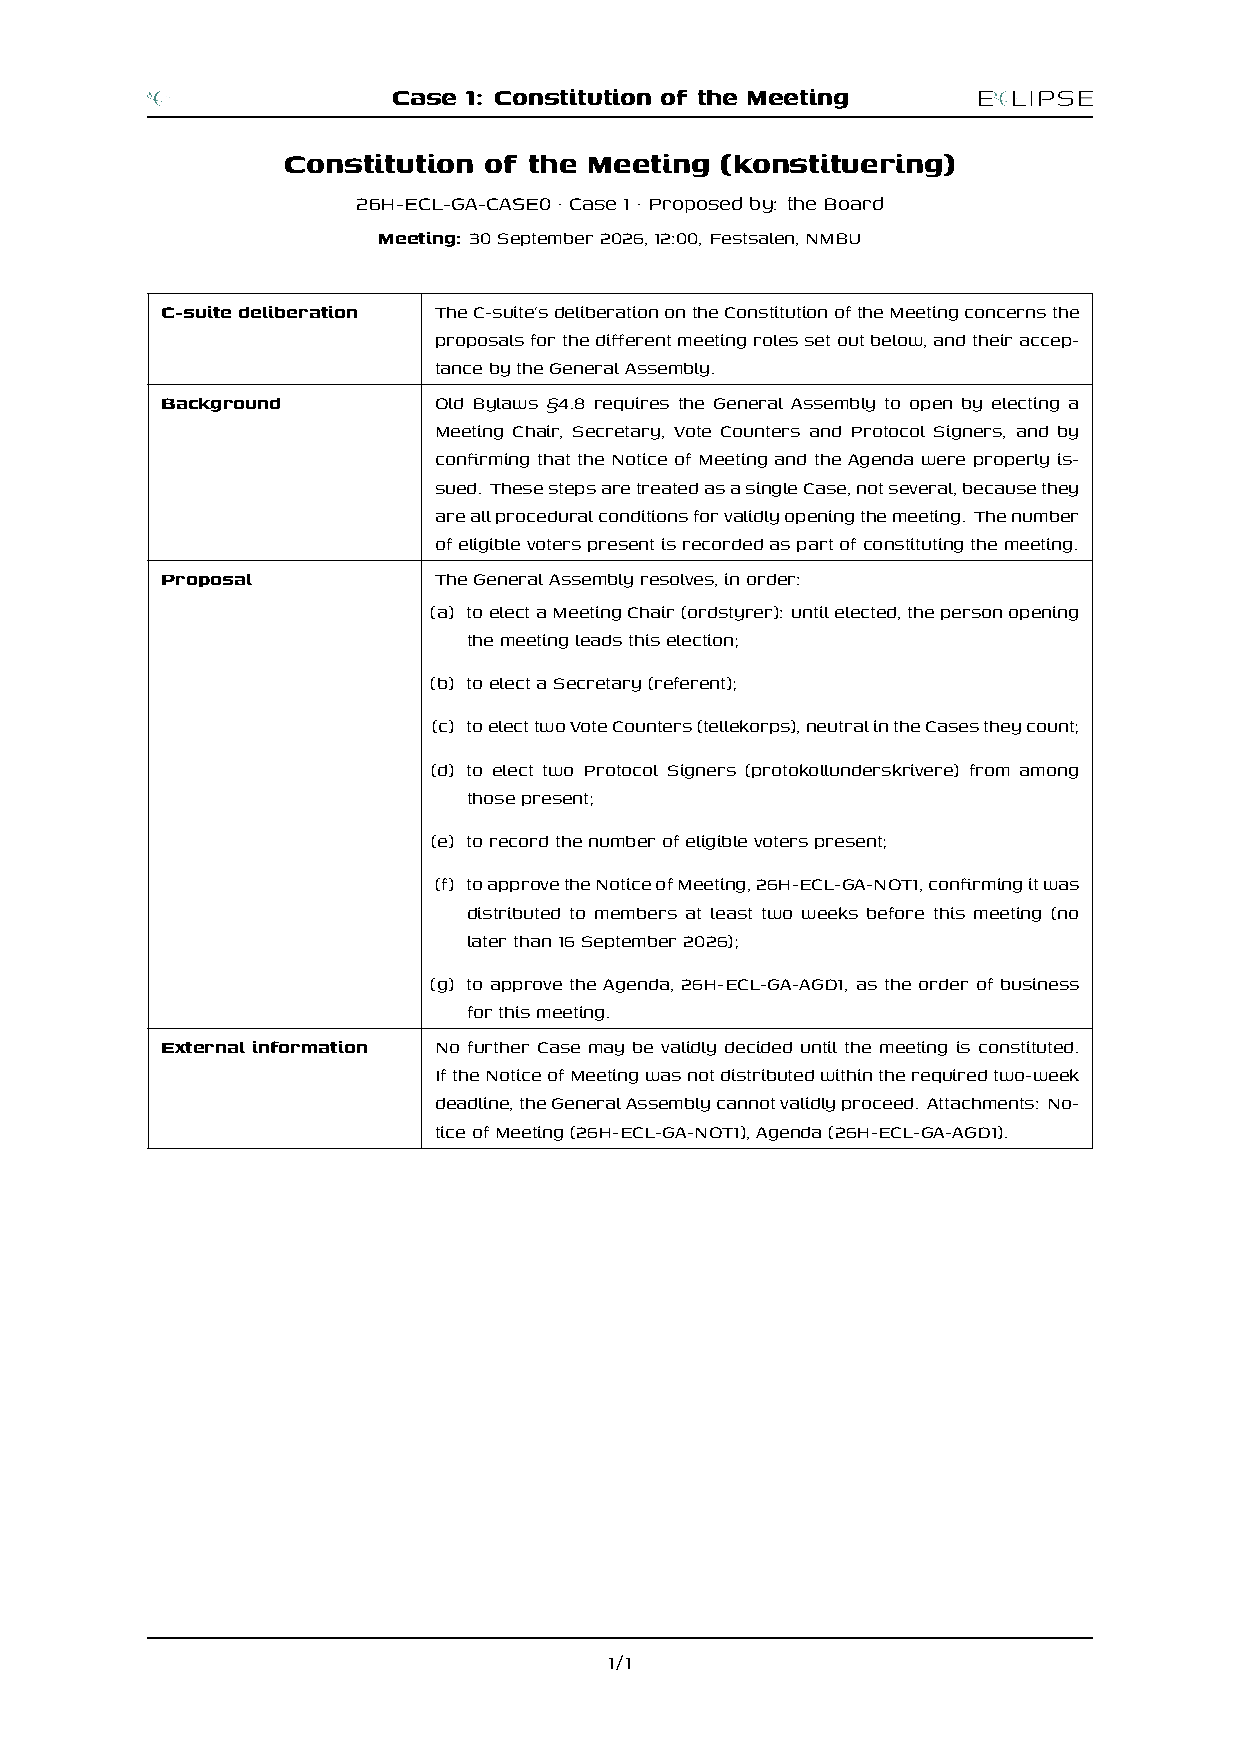
\includepdf[pages=-]{../05 Standard Case Papers/26H-ECL-GA-CASE0.pdf}
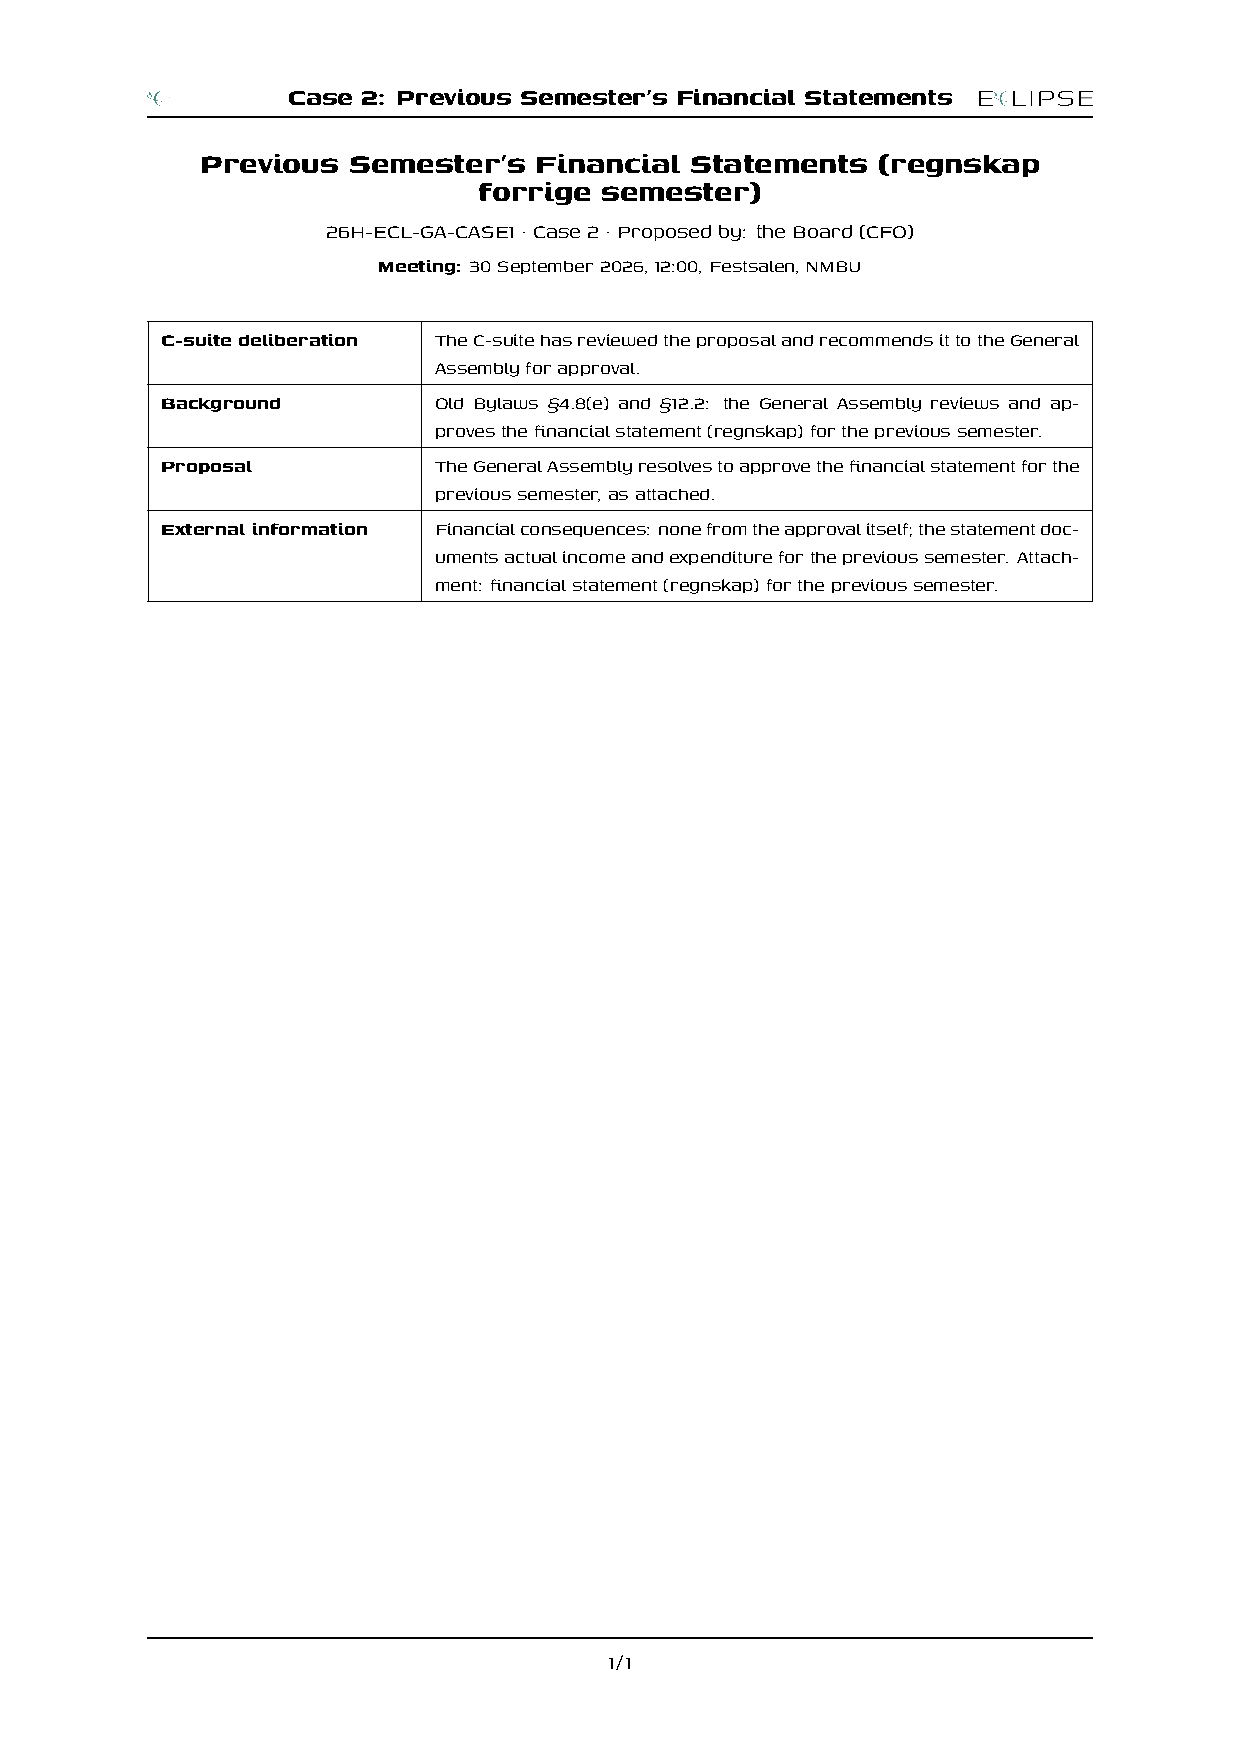
\includepdf[pages=-]{../05 Standard Case Papers/26H-ECL-GA-CASE1.pdf}
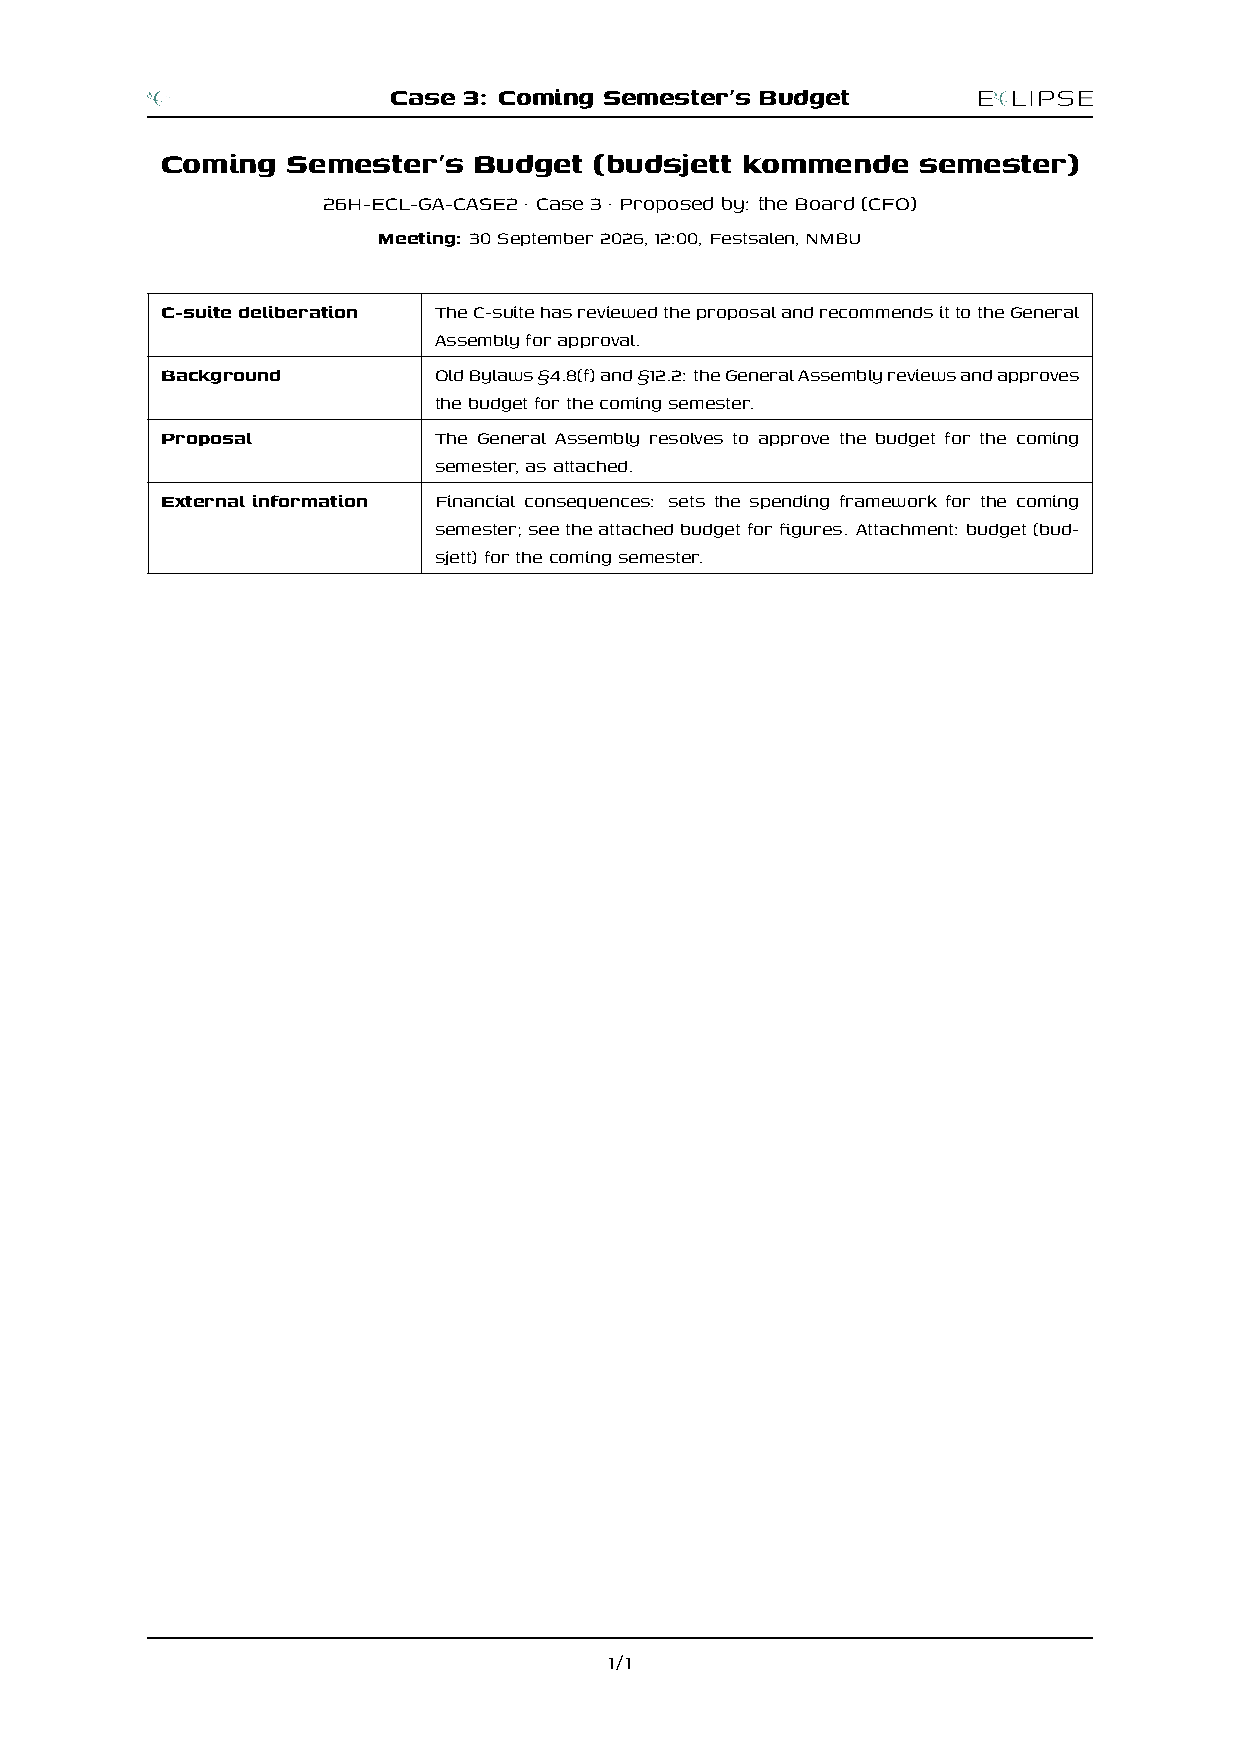
\includepdf[pages=-]{../05 Standard Case Papers/26H-ECL-GA-CASE2.pdf}
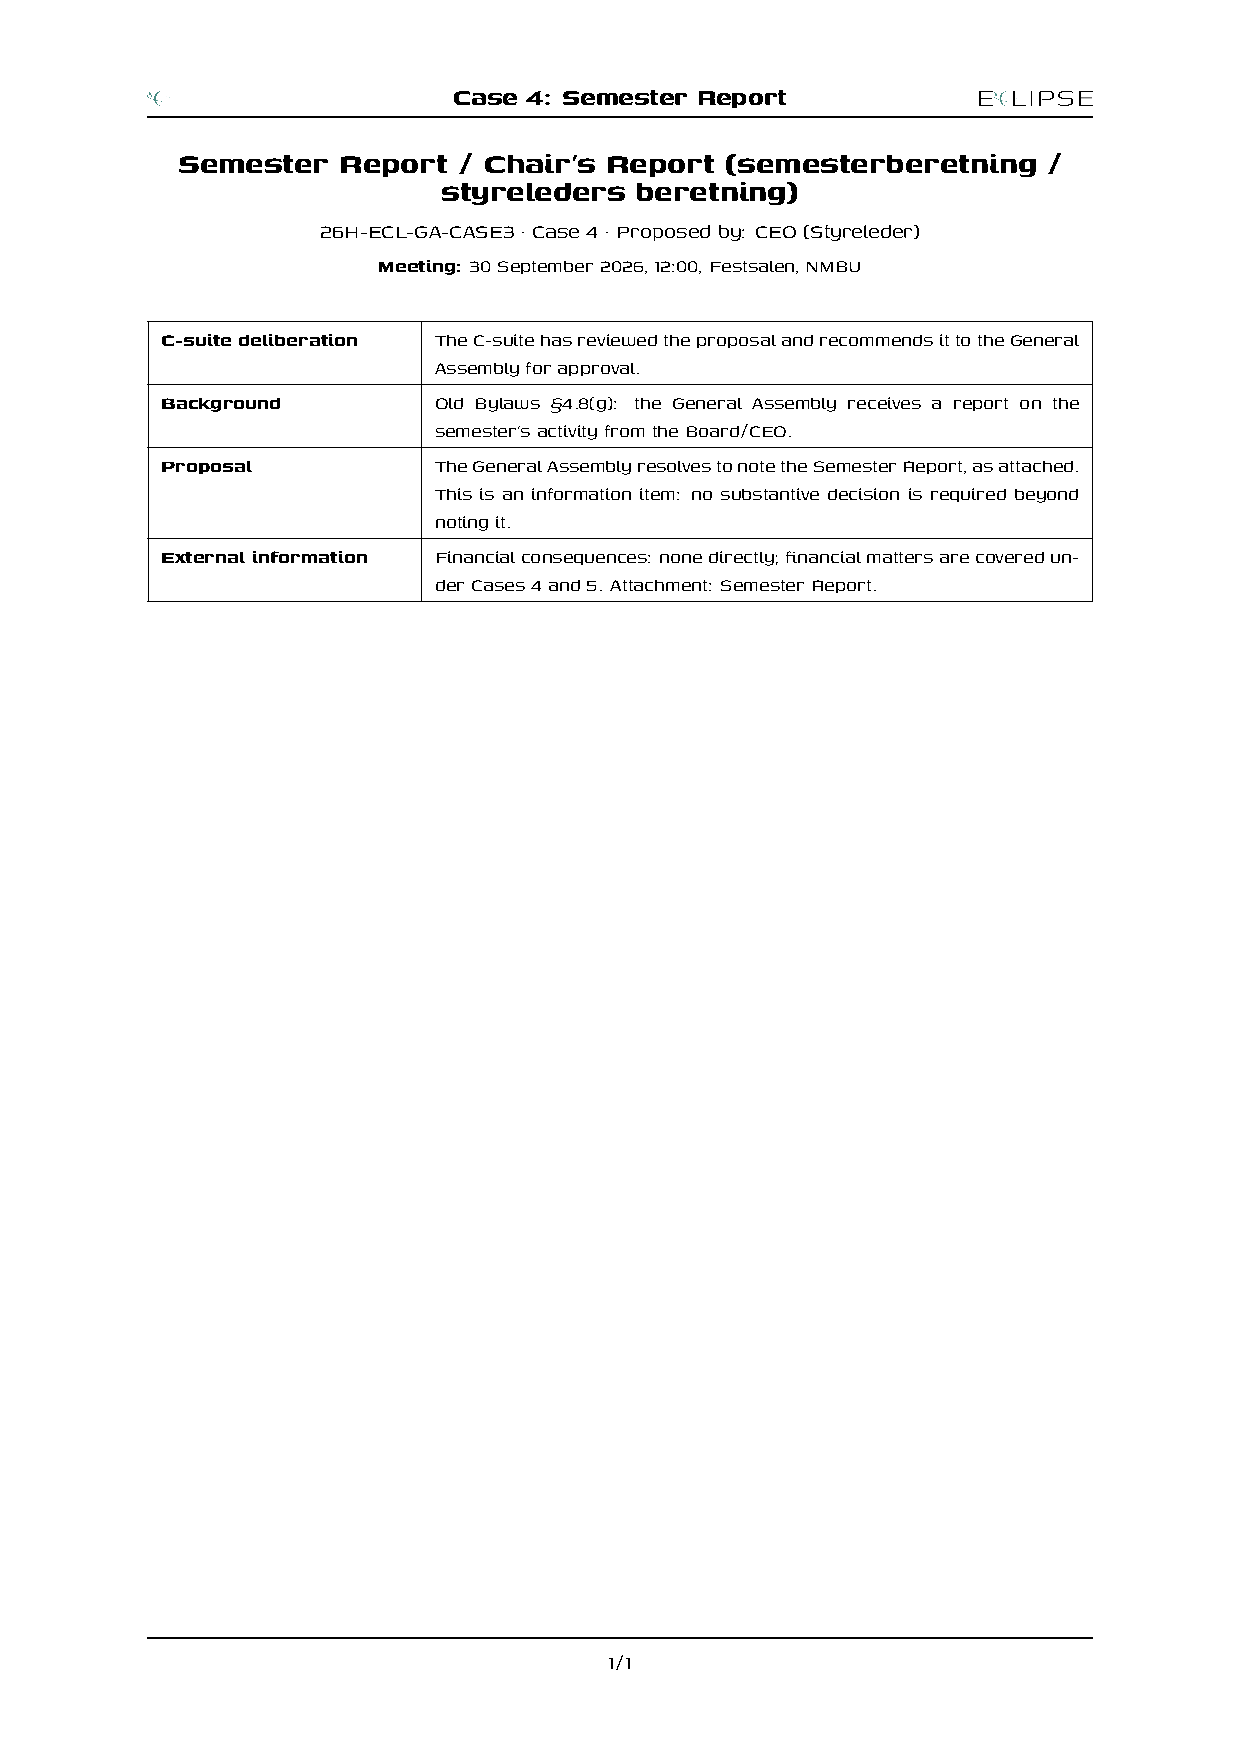
\includepdf[pages=-]{../05 Standard Case Papers/26H-ECL-GA-CASE3.pdf}
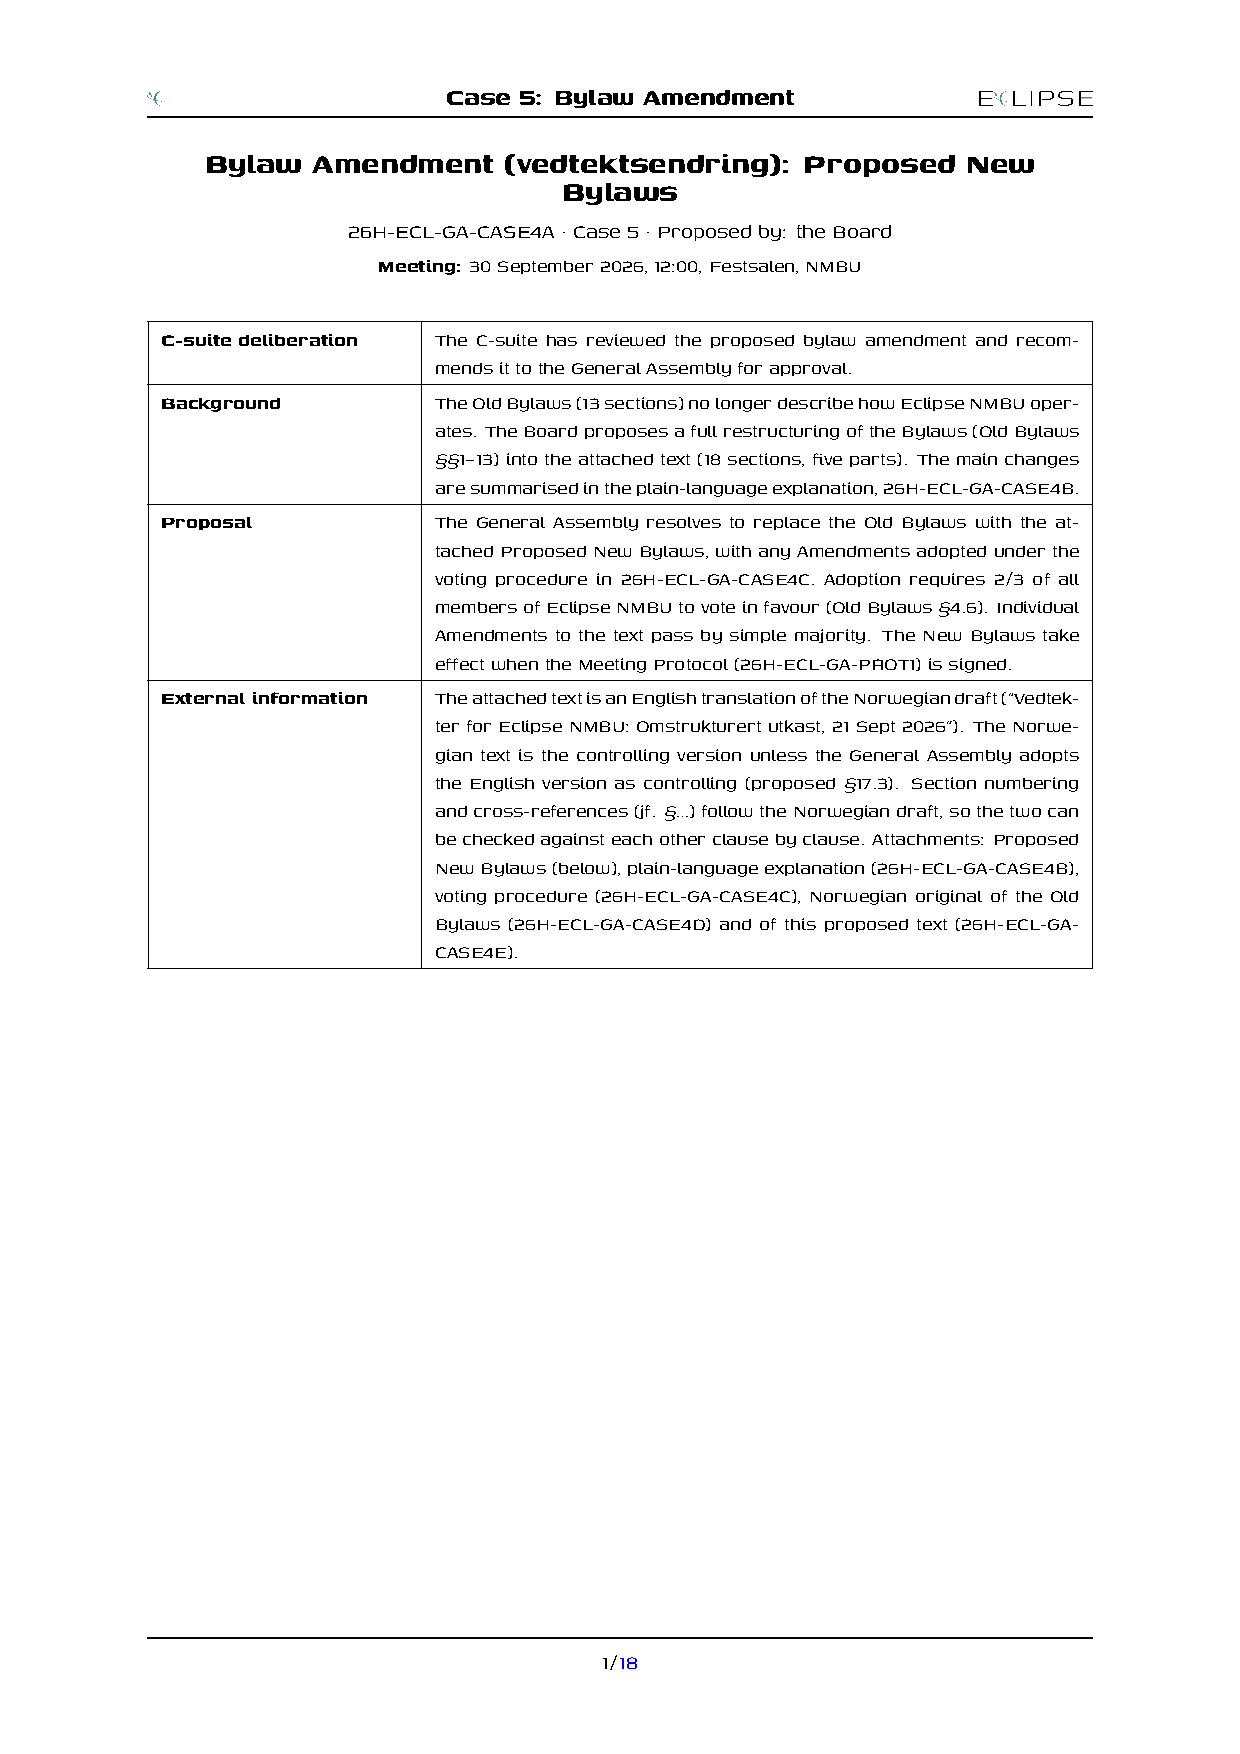
\includepdf[pages=-]{../06 Bylaw Amendment Proposal/26H-ECL-GA-CASE4A.pdf}

\includepdf[pages=-]{../06 Bylaw Amendment Proposal/26H-ECL-GA-CASE4B.pdf}

\includepdf[pages=-]{../06 Bylaw Amendment Proposal/26H-ECL-GA-CASE4C.pdf}
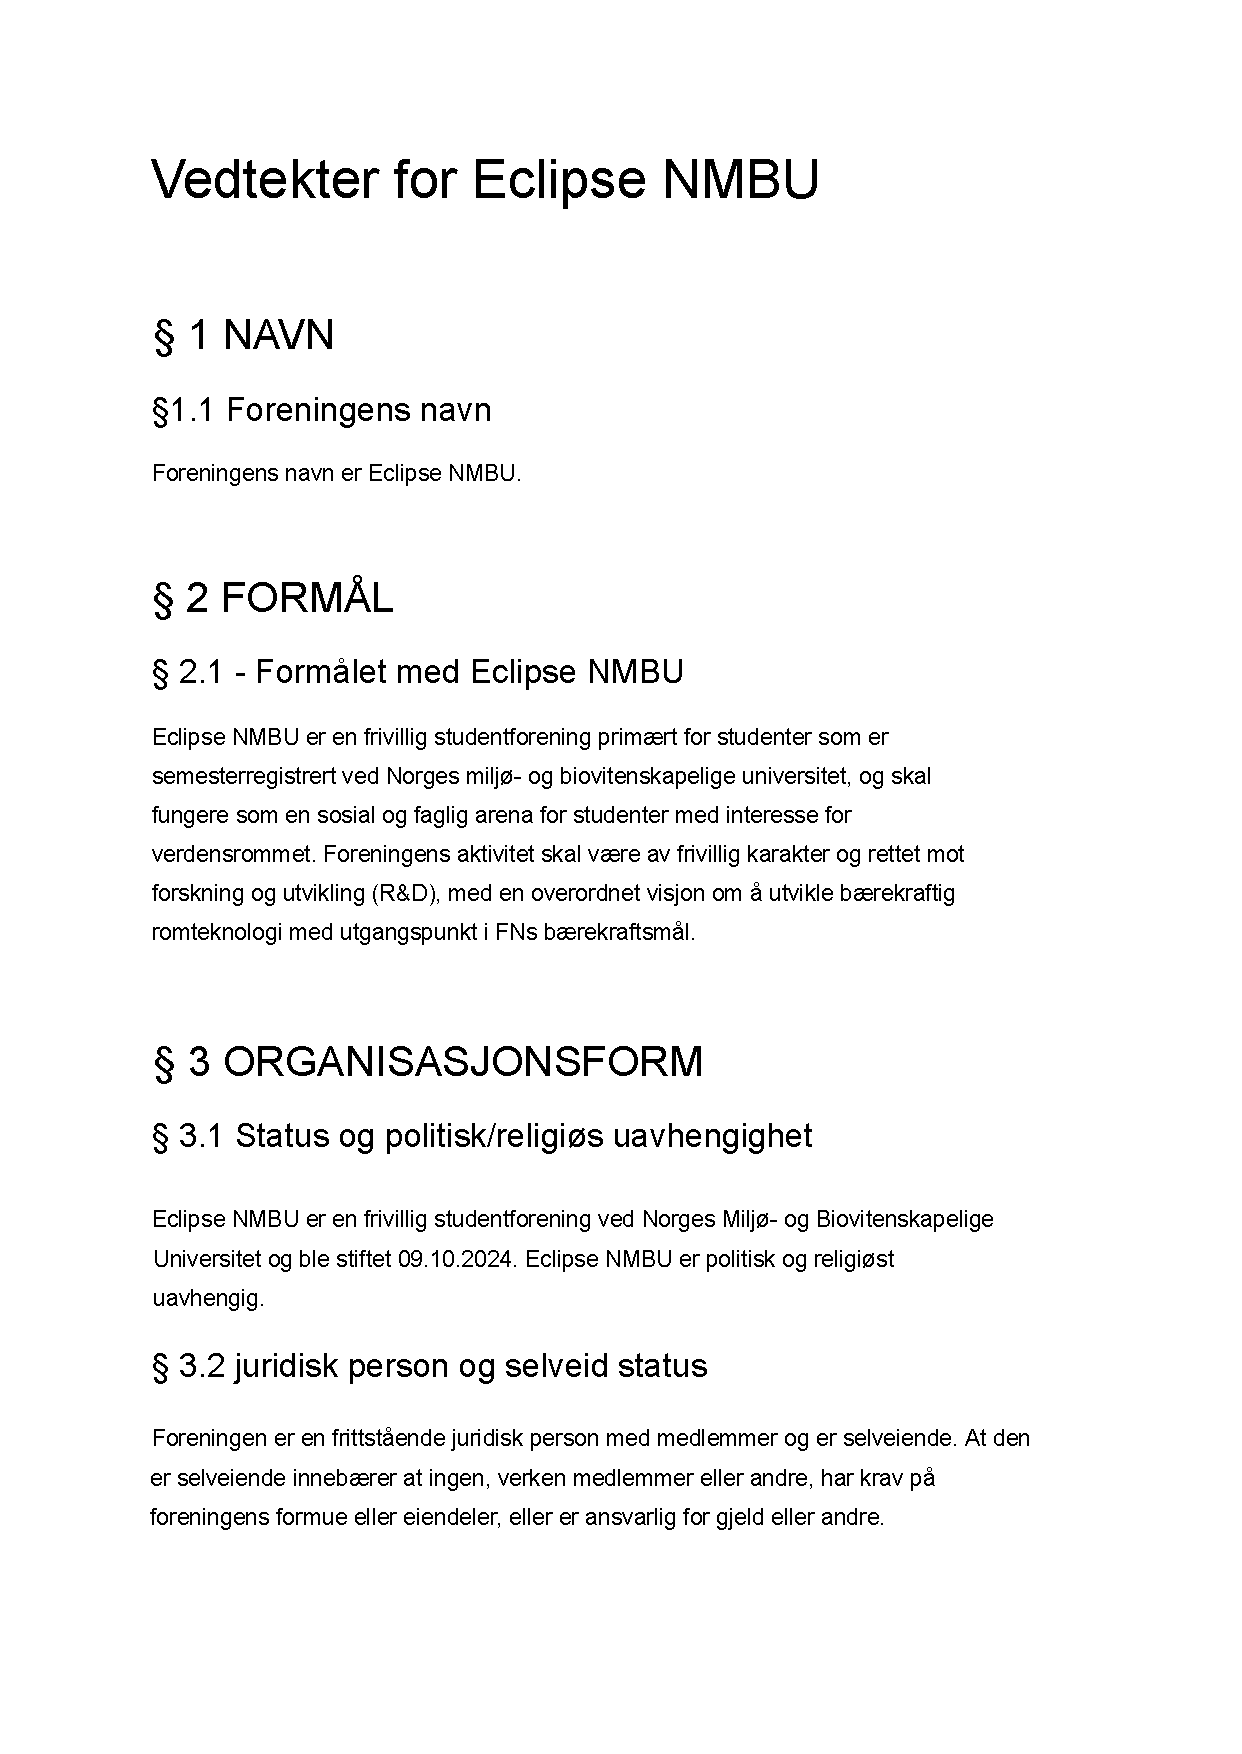
\includepdf[pages=-]{../06 Bylaw Amendment Proposal/26H-ECL-GA-CASE4D.pdf}
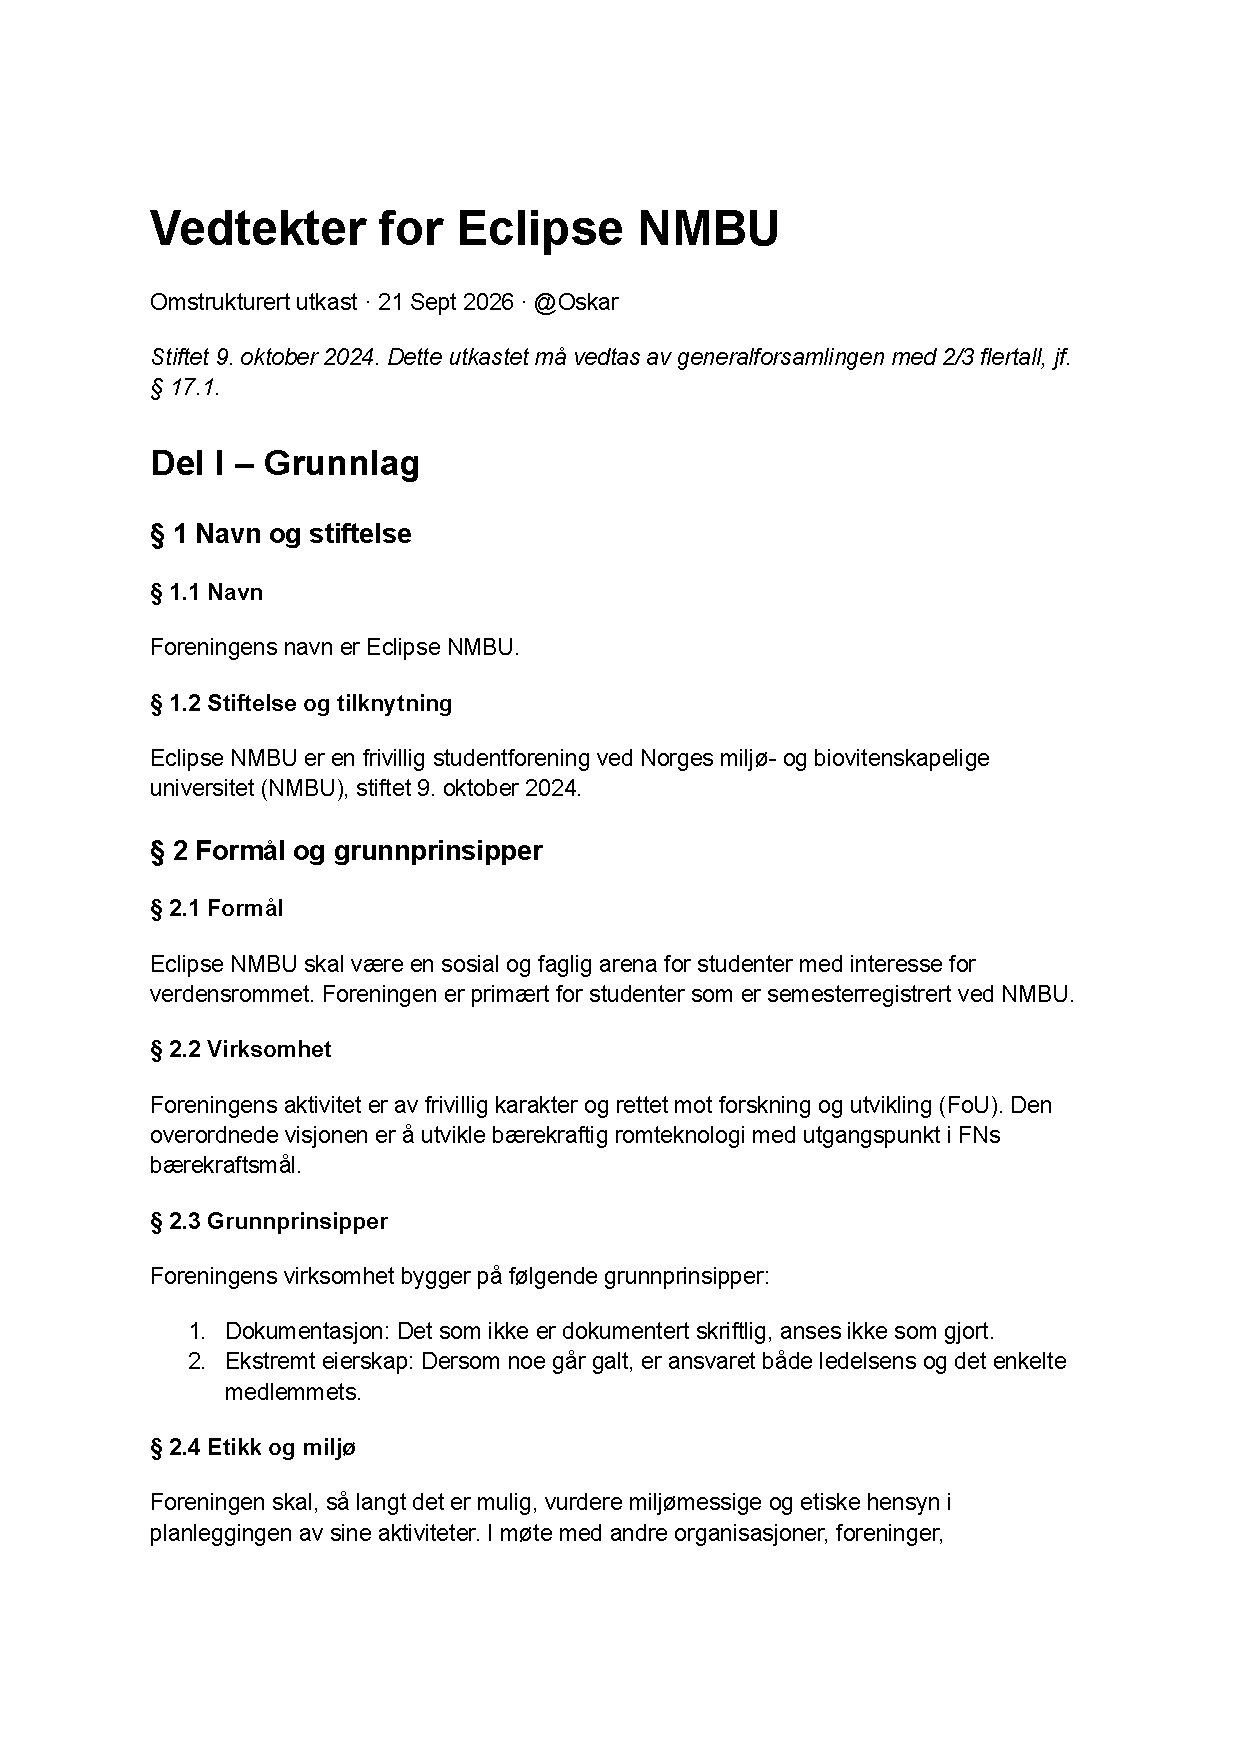
\includepdf[pages=-]{../06 Bylaw Amendment Proposal/26H-ECL-GA-CASE4E.pdf}
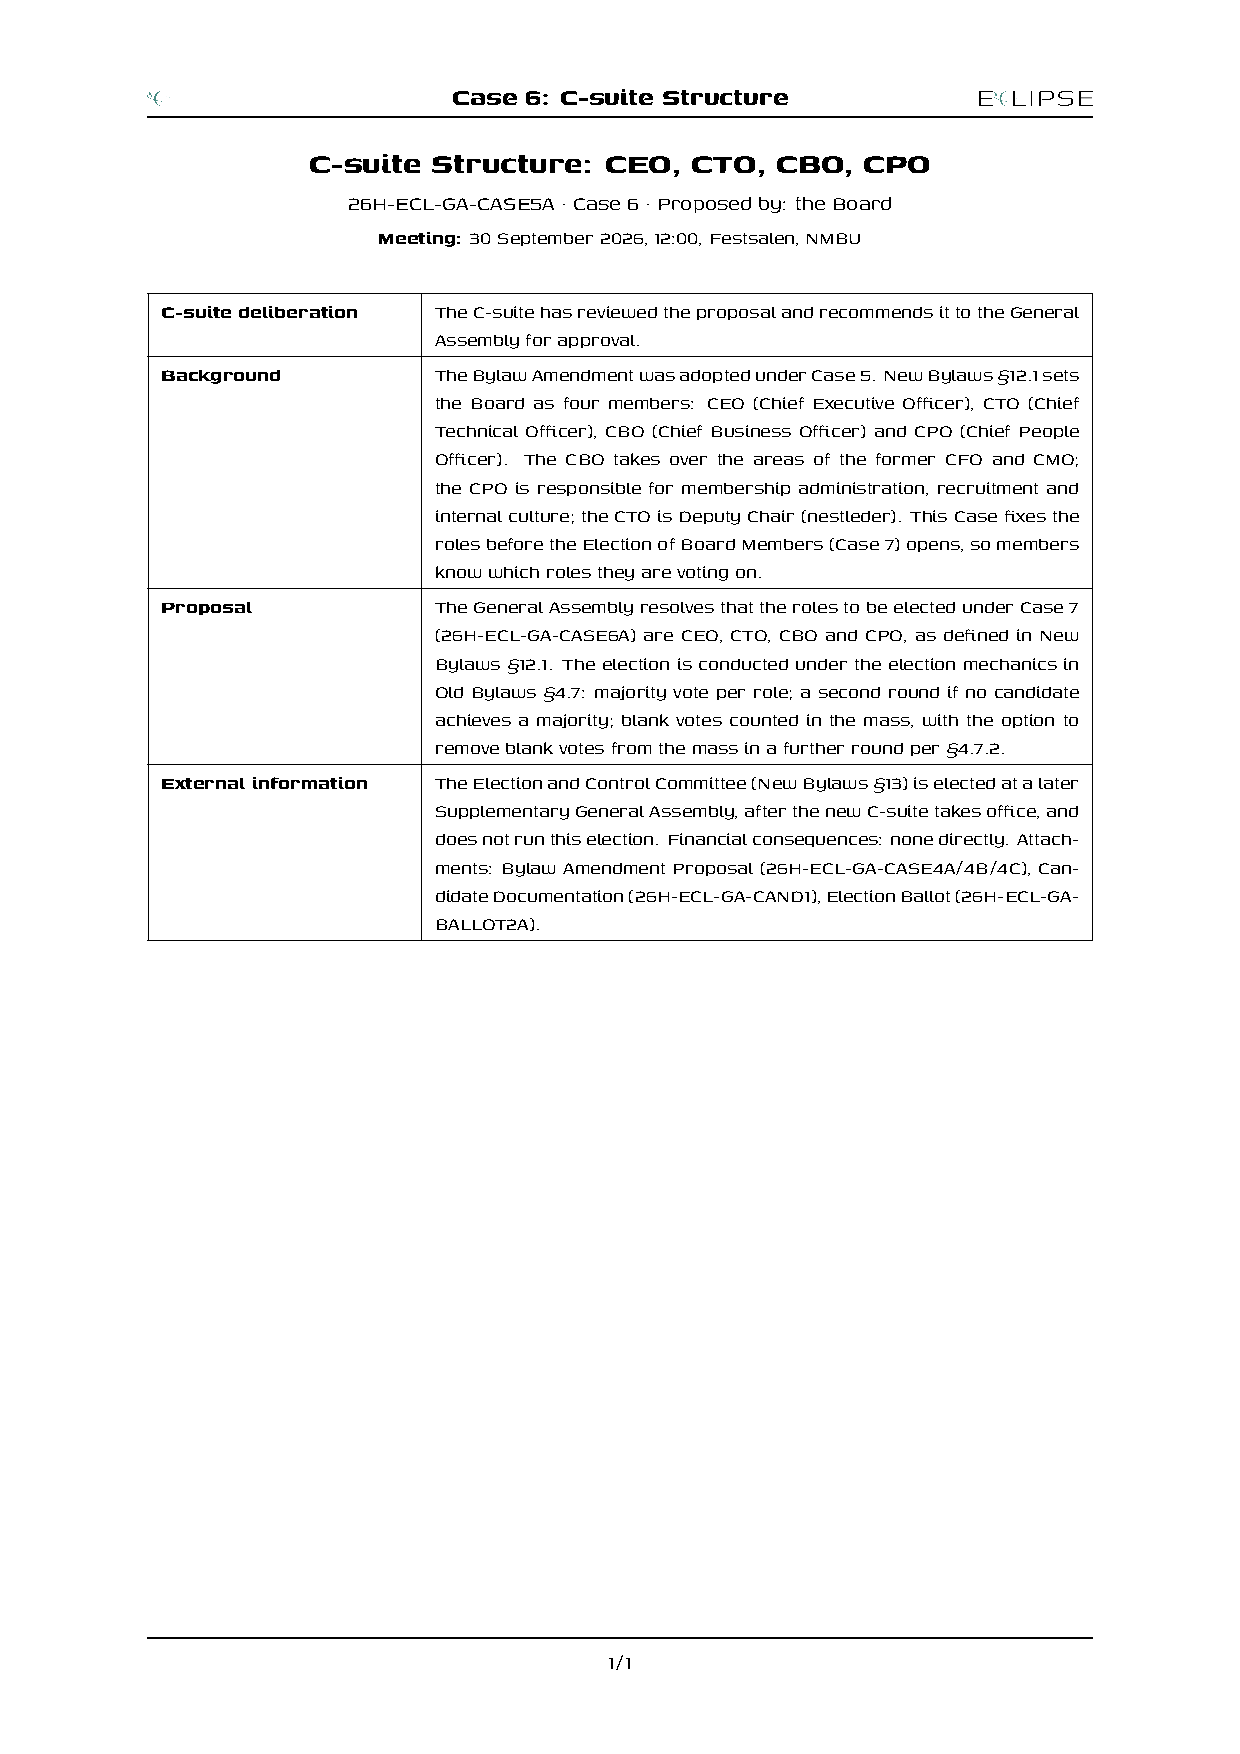
\includepdf[pages=-]{../07 Transitional C-suite Case/26H-ECL-GA-CASE5A.pdf}
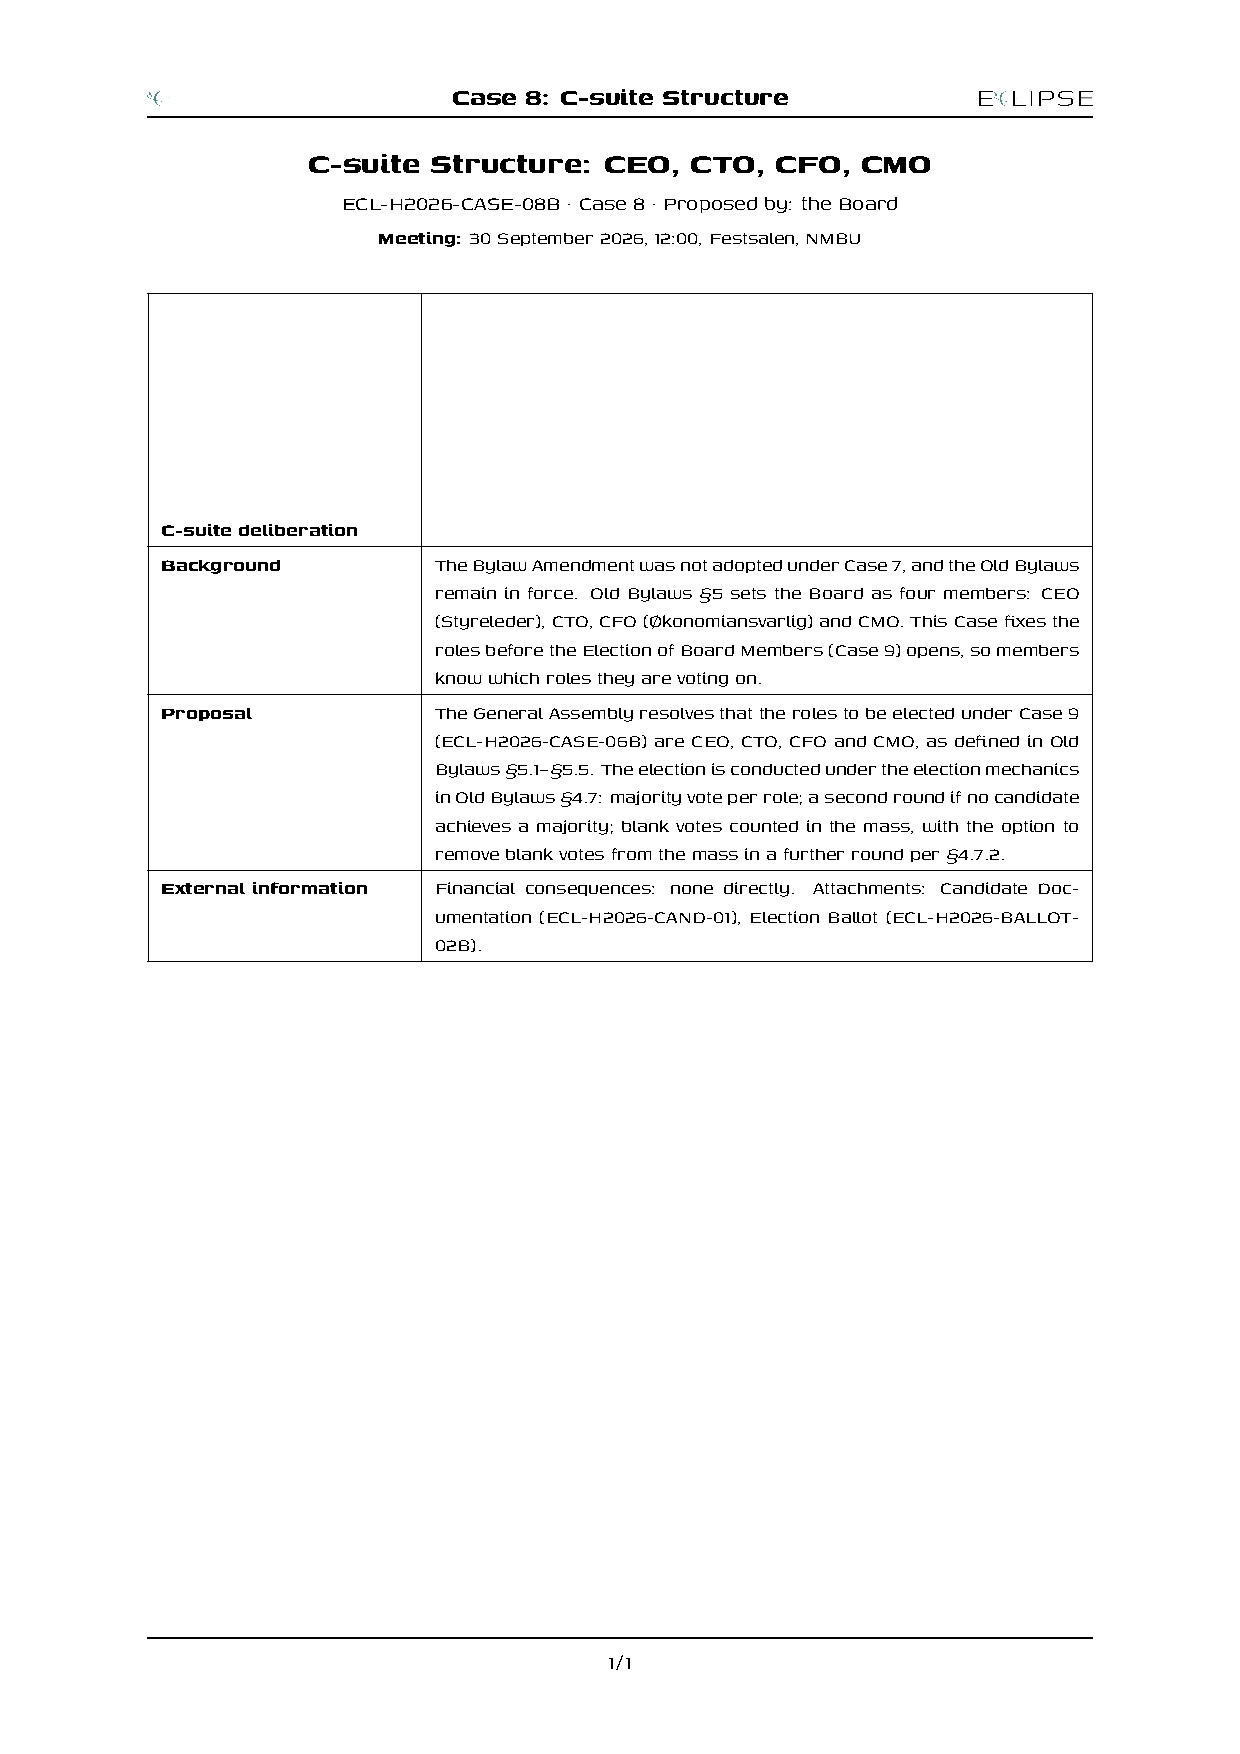
\includepdf[pages=-]{../07 Transitional C-suite Case/26H-ECL-GA-CASE5B.pdf}
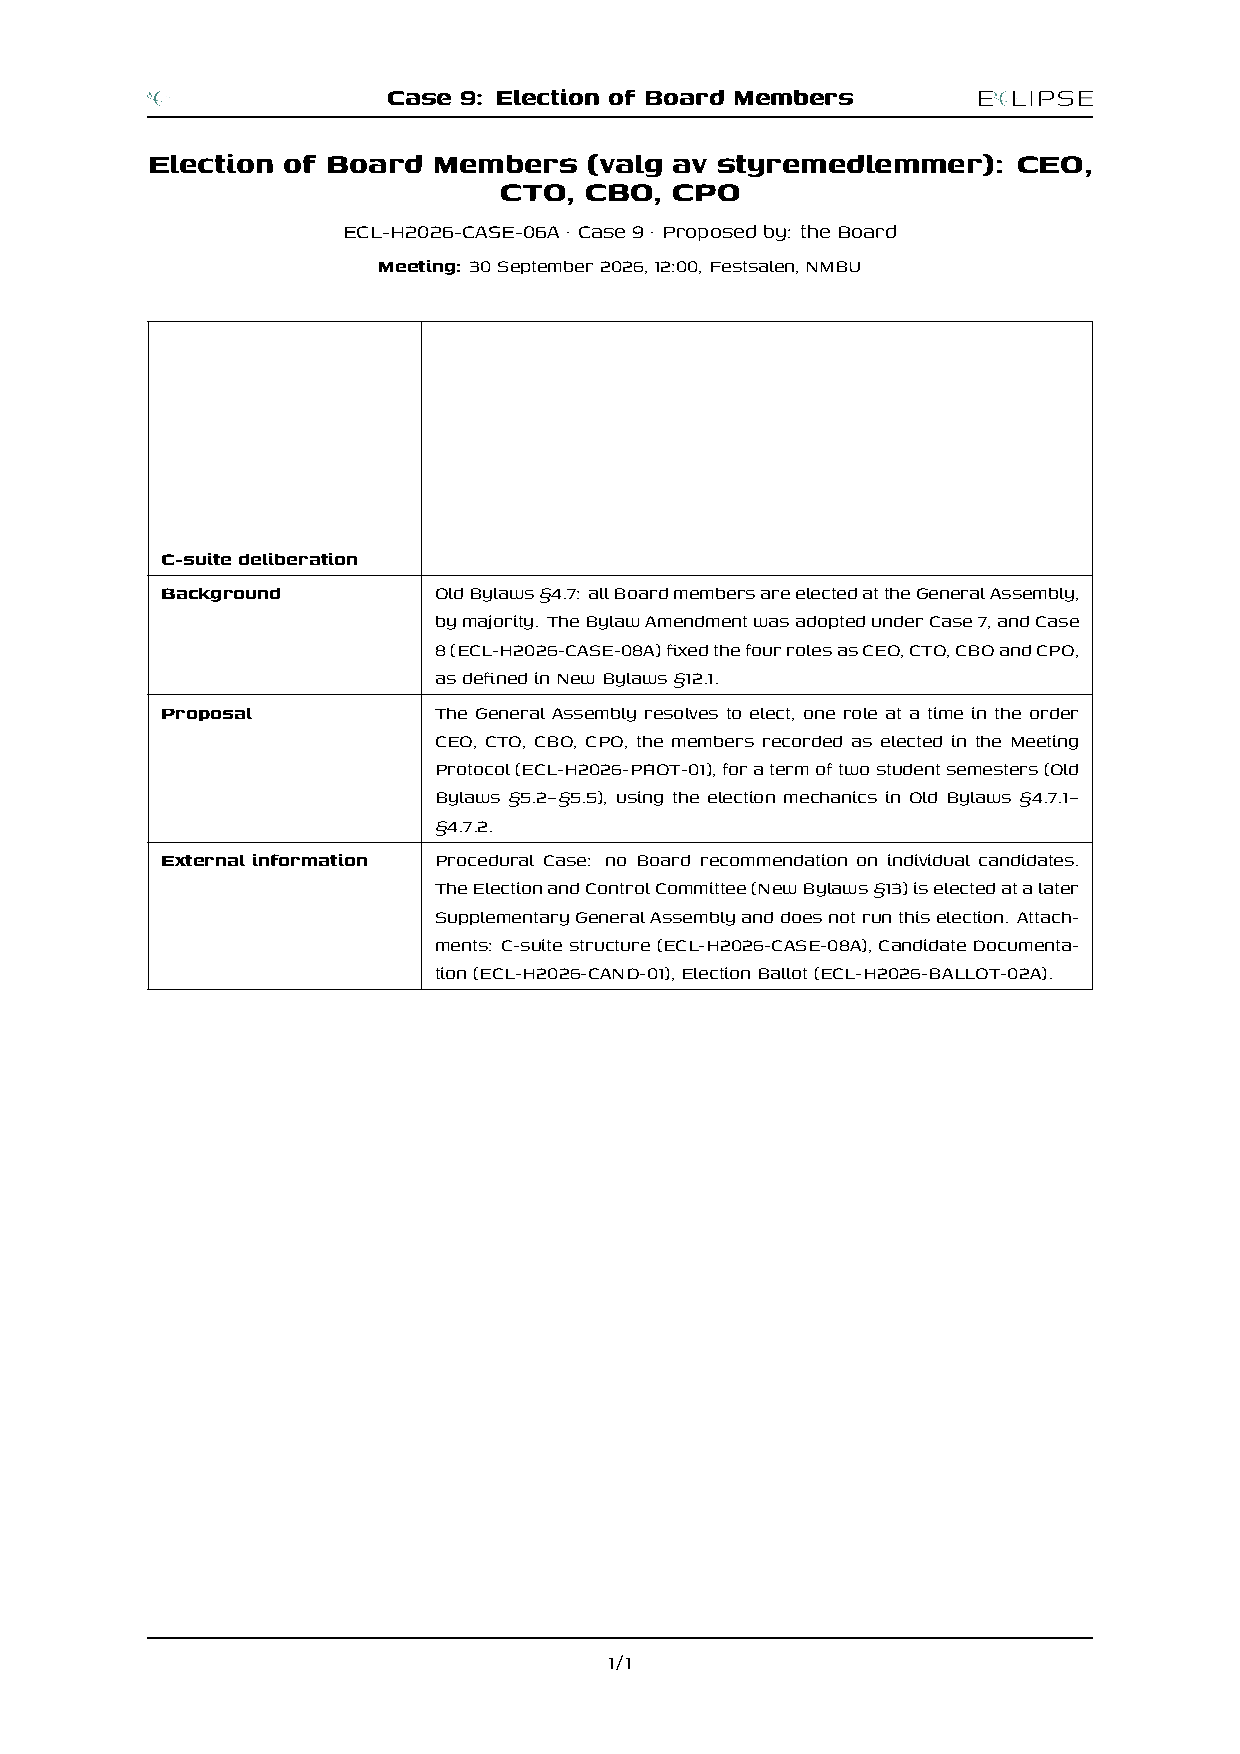
\includepdf[pages=-]{../05 Standard Case Papers/26H-ECL-GA-CASE6A.pdf}
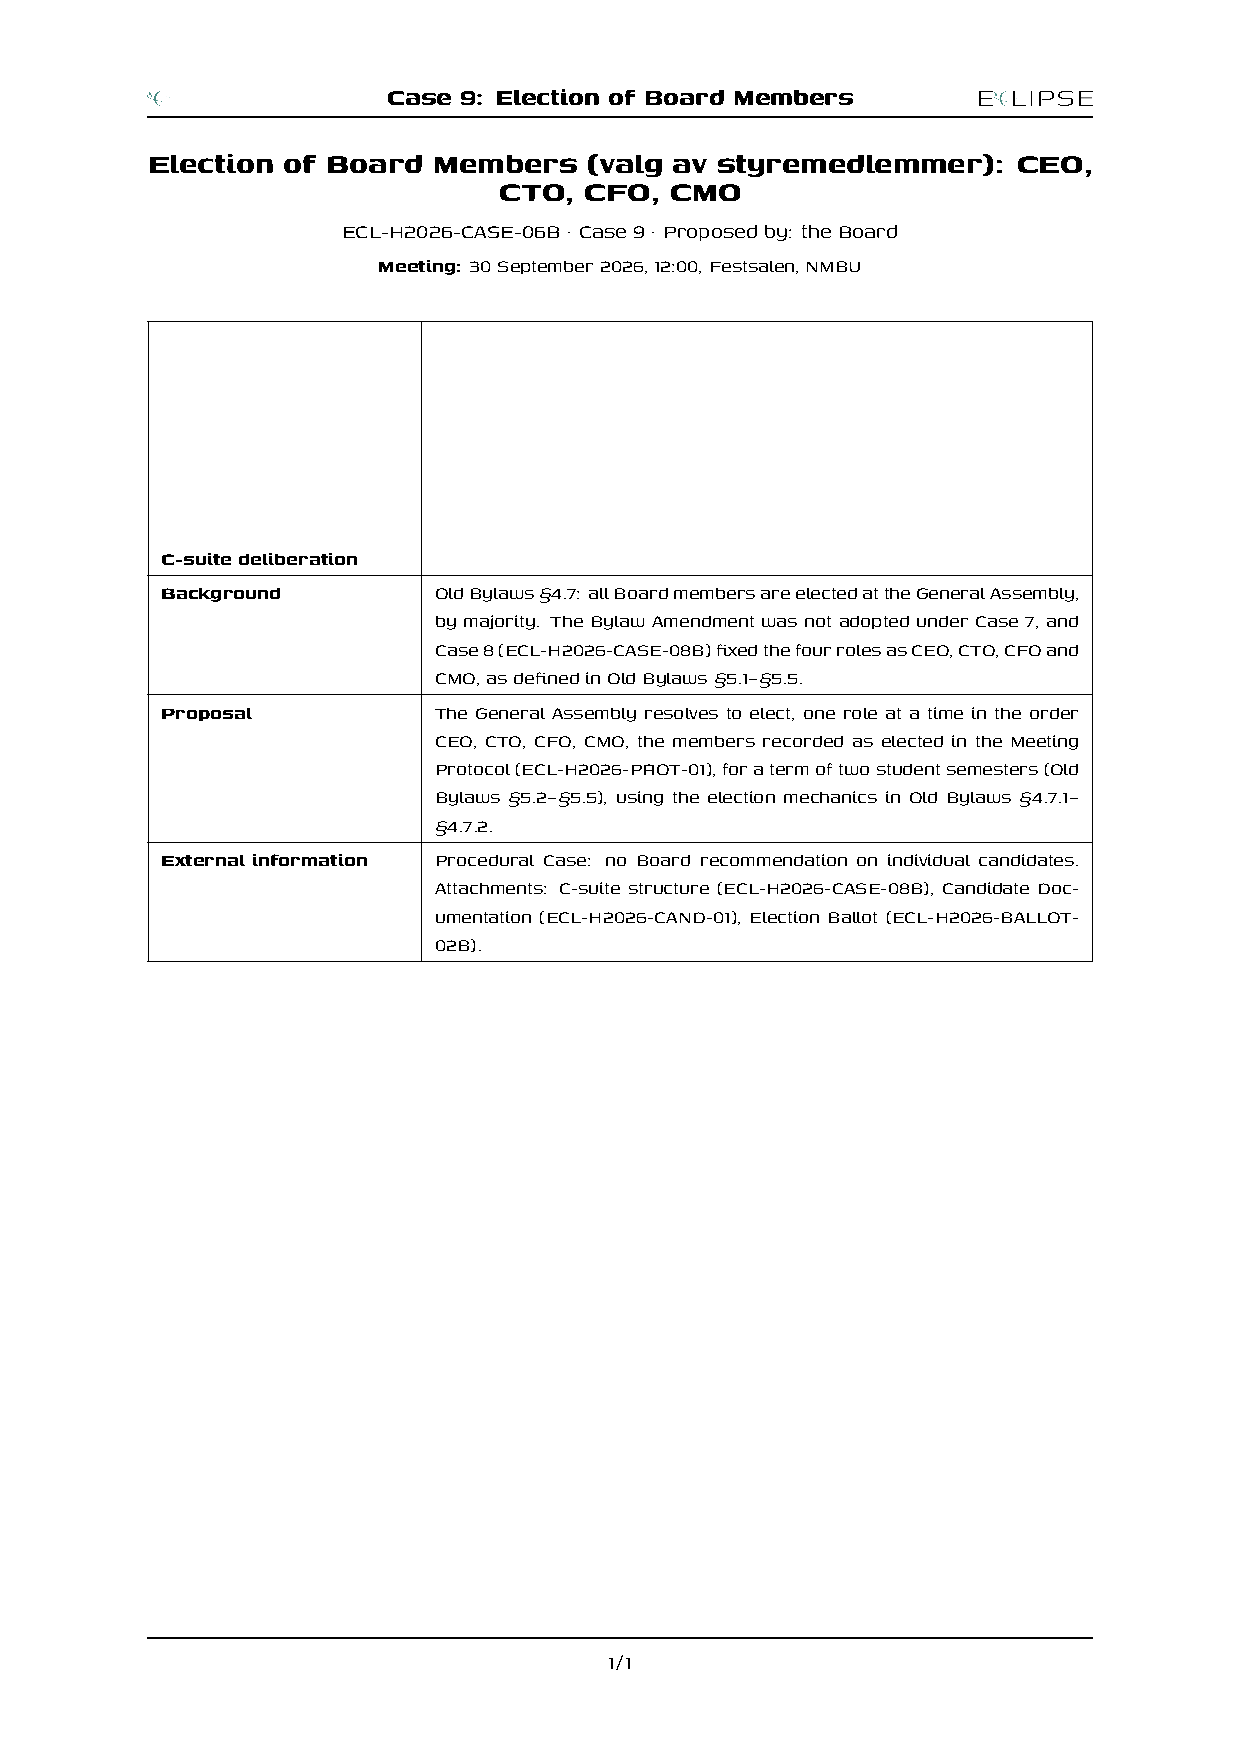
\includepdf[pages=-]{../05 Standard Case Papers/26H-ECL-GA-CASE6B.pdf}
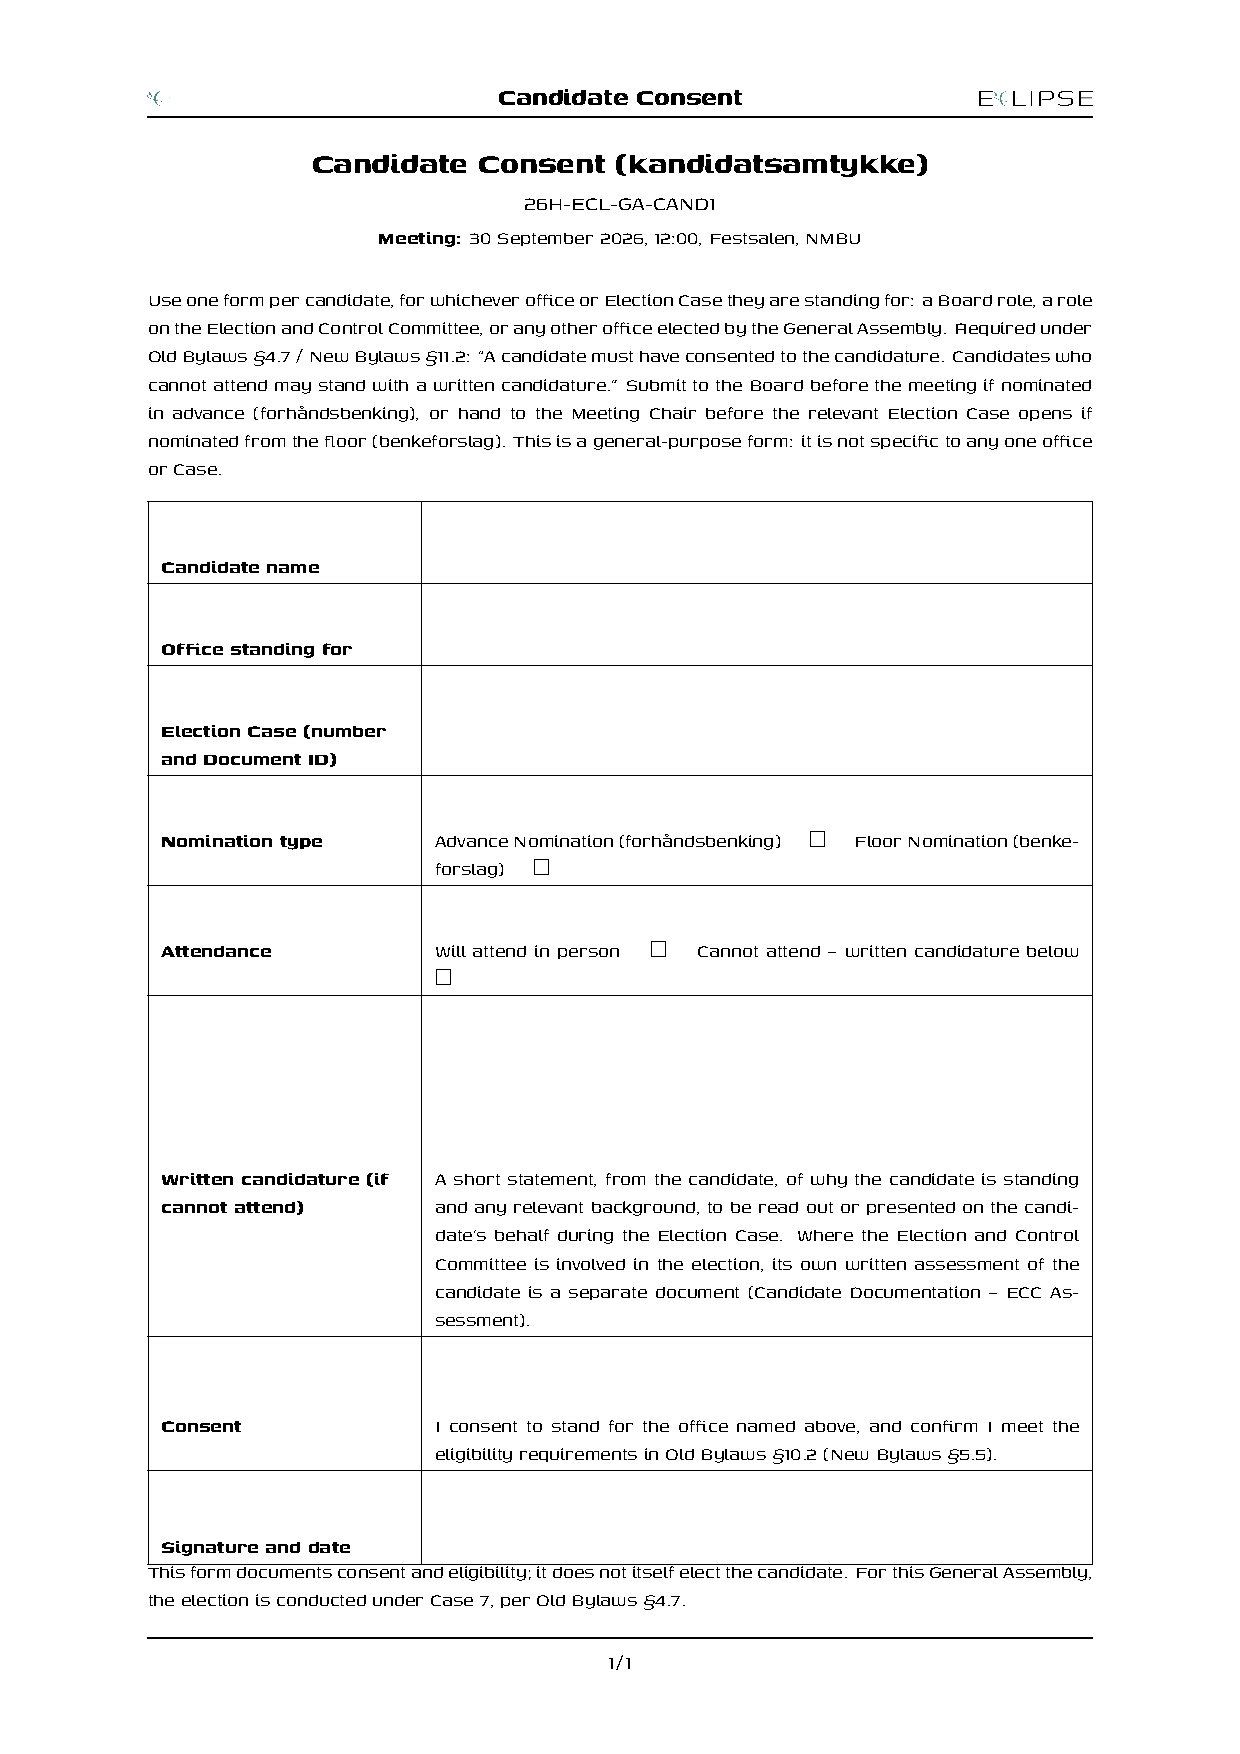
\includepdf[pages=-]{../08 Candidate Documentation/26H-ECL-GA-CAND1.pdf}
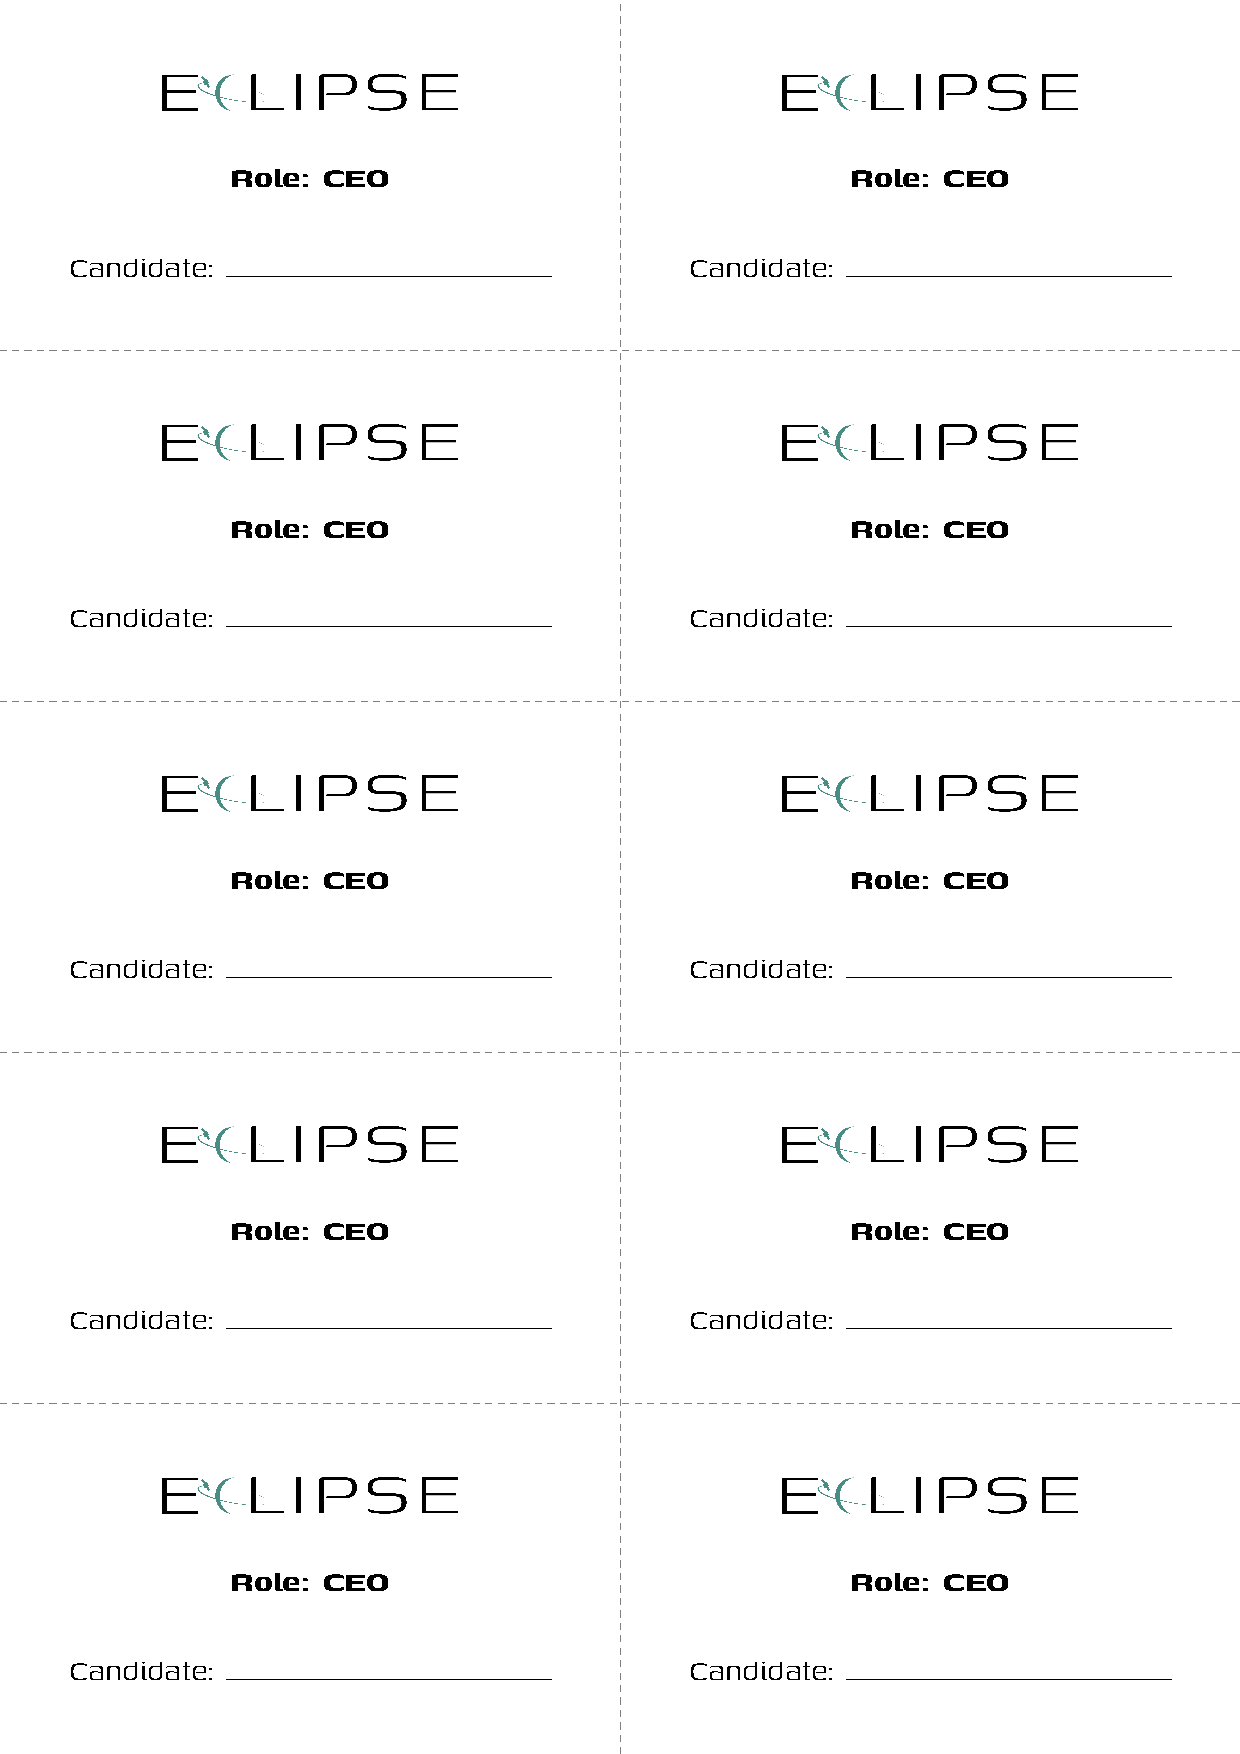
\includepdf[pages=-]{../10 Election Ballots/26H-ECL-GA-BALLOT2A.pdf}
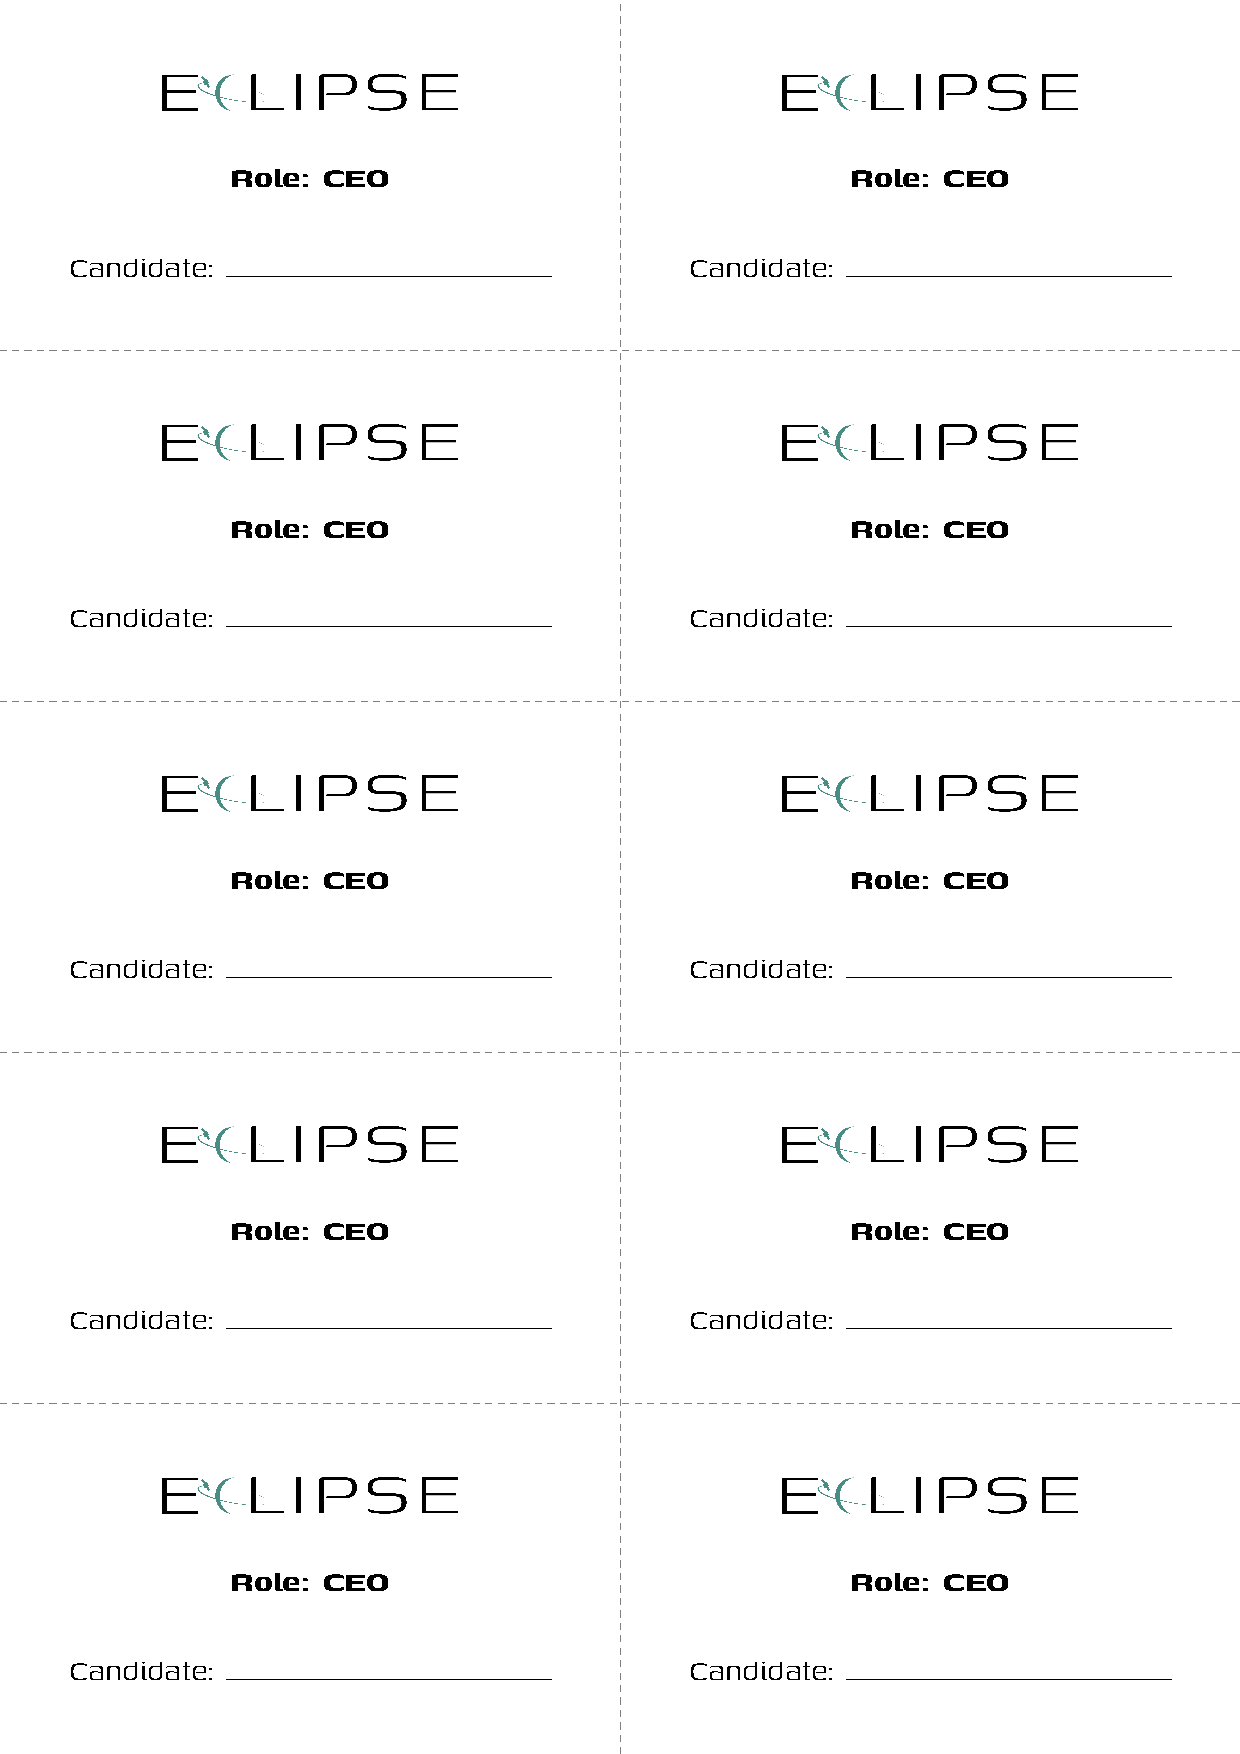
\includepdf[pages=-]{../10 Election Ballots/26H-ECL-GA-BALLOT2B.pdf}

\includepdf[pages=-]{../11 Voting Order/26H-ECL-GA-VOTORD1.pdf}

\includepdf[pages=-]{../12 Meeting Protocol/26H-ECL-GA-PROT1.pdf}

\includepdf[pages=-]{../13 Membership Contract/26H-ECL-GA-MEMB1.pdf}
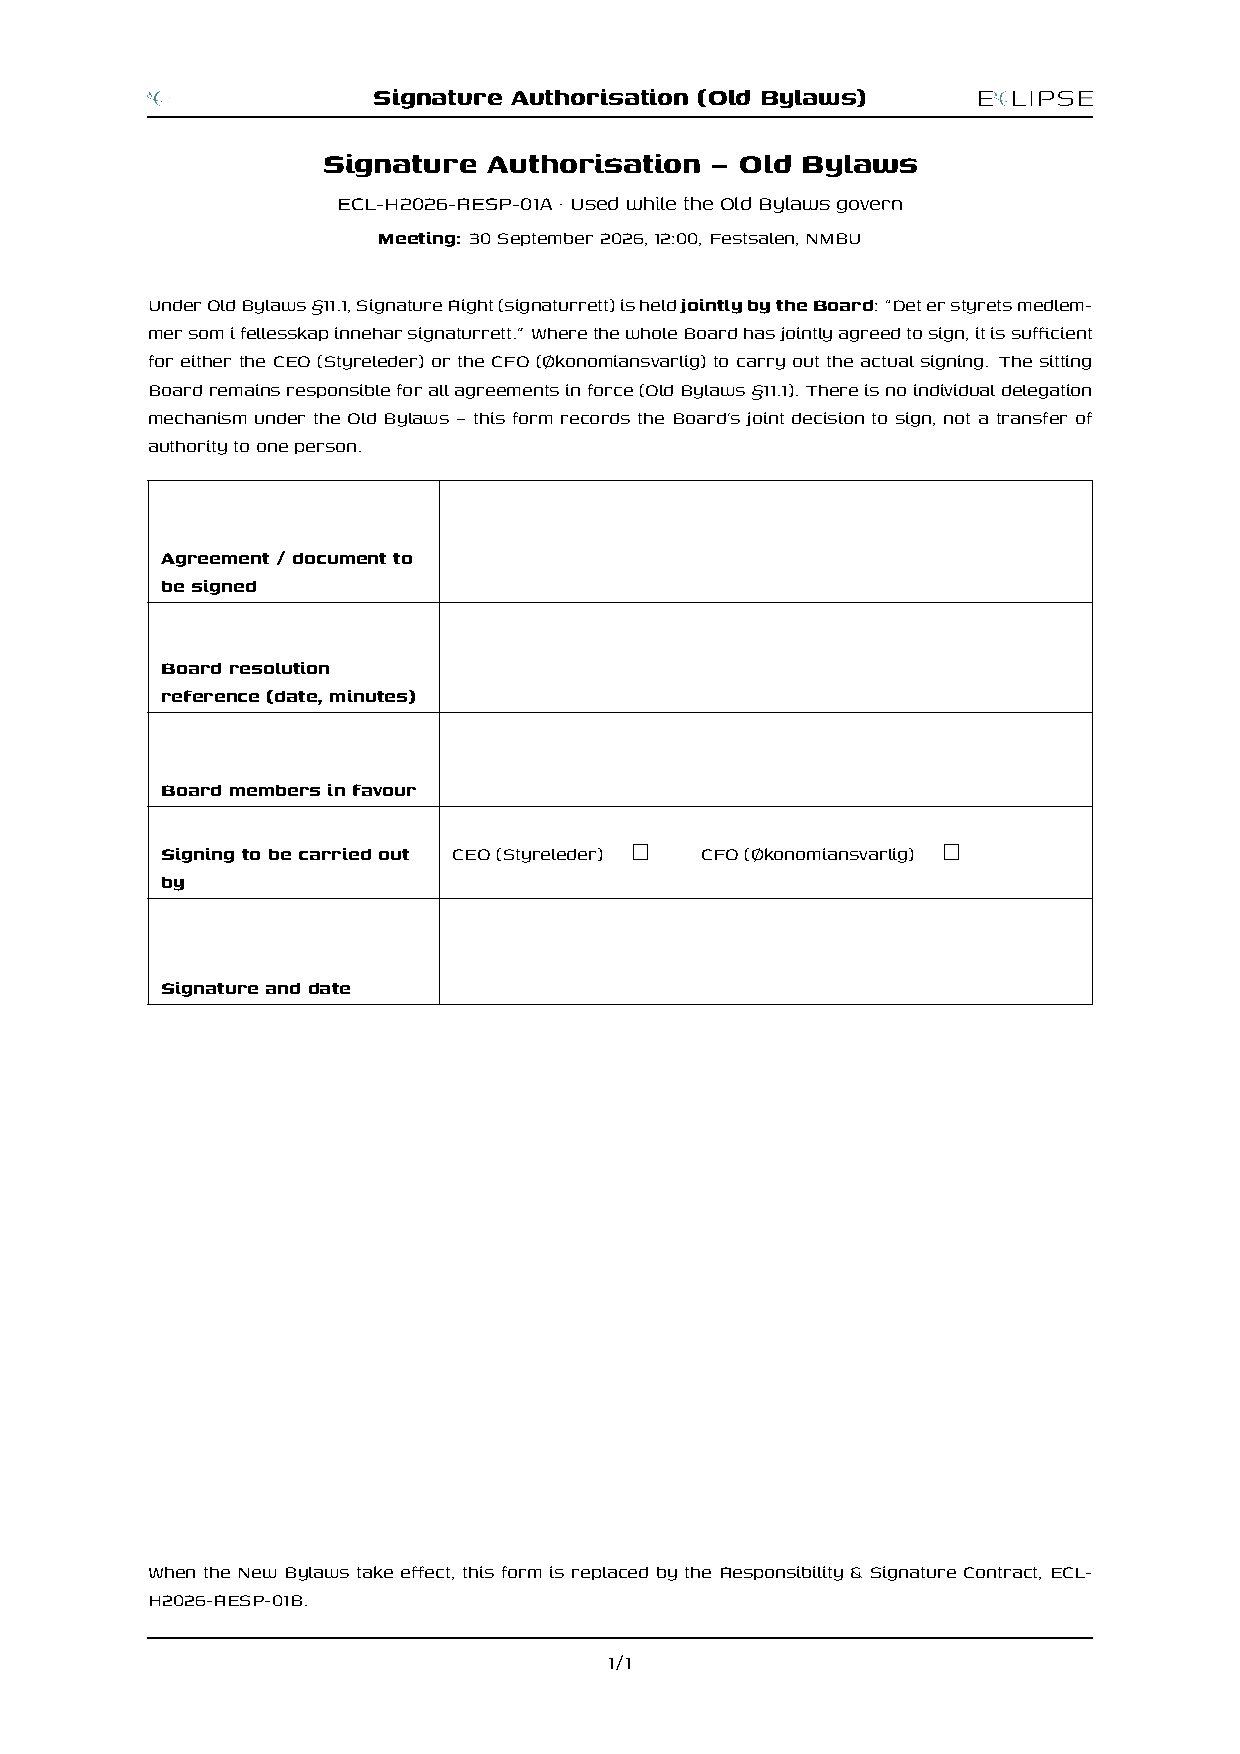
\includepdf[pages=-]{../14 Responsibility and Signature Contract/26H-ECL-GA-RESP1A.pdf}

\includepdf[pages=-]{../14 Responsibility and Signature Contract/26H-ECL-GA-RESP1B.pdf}
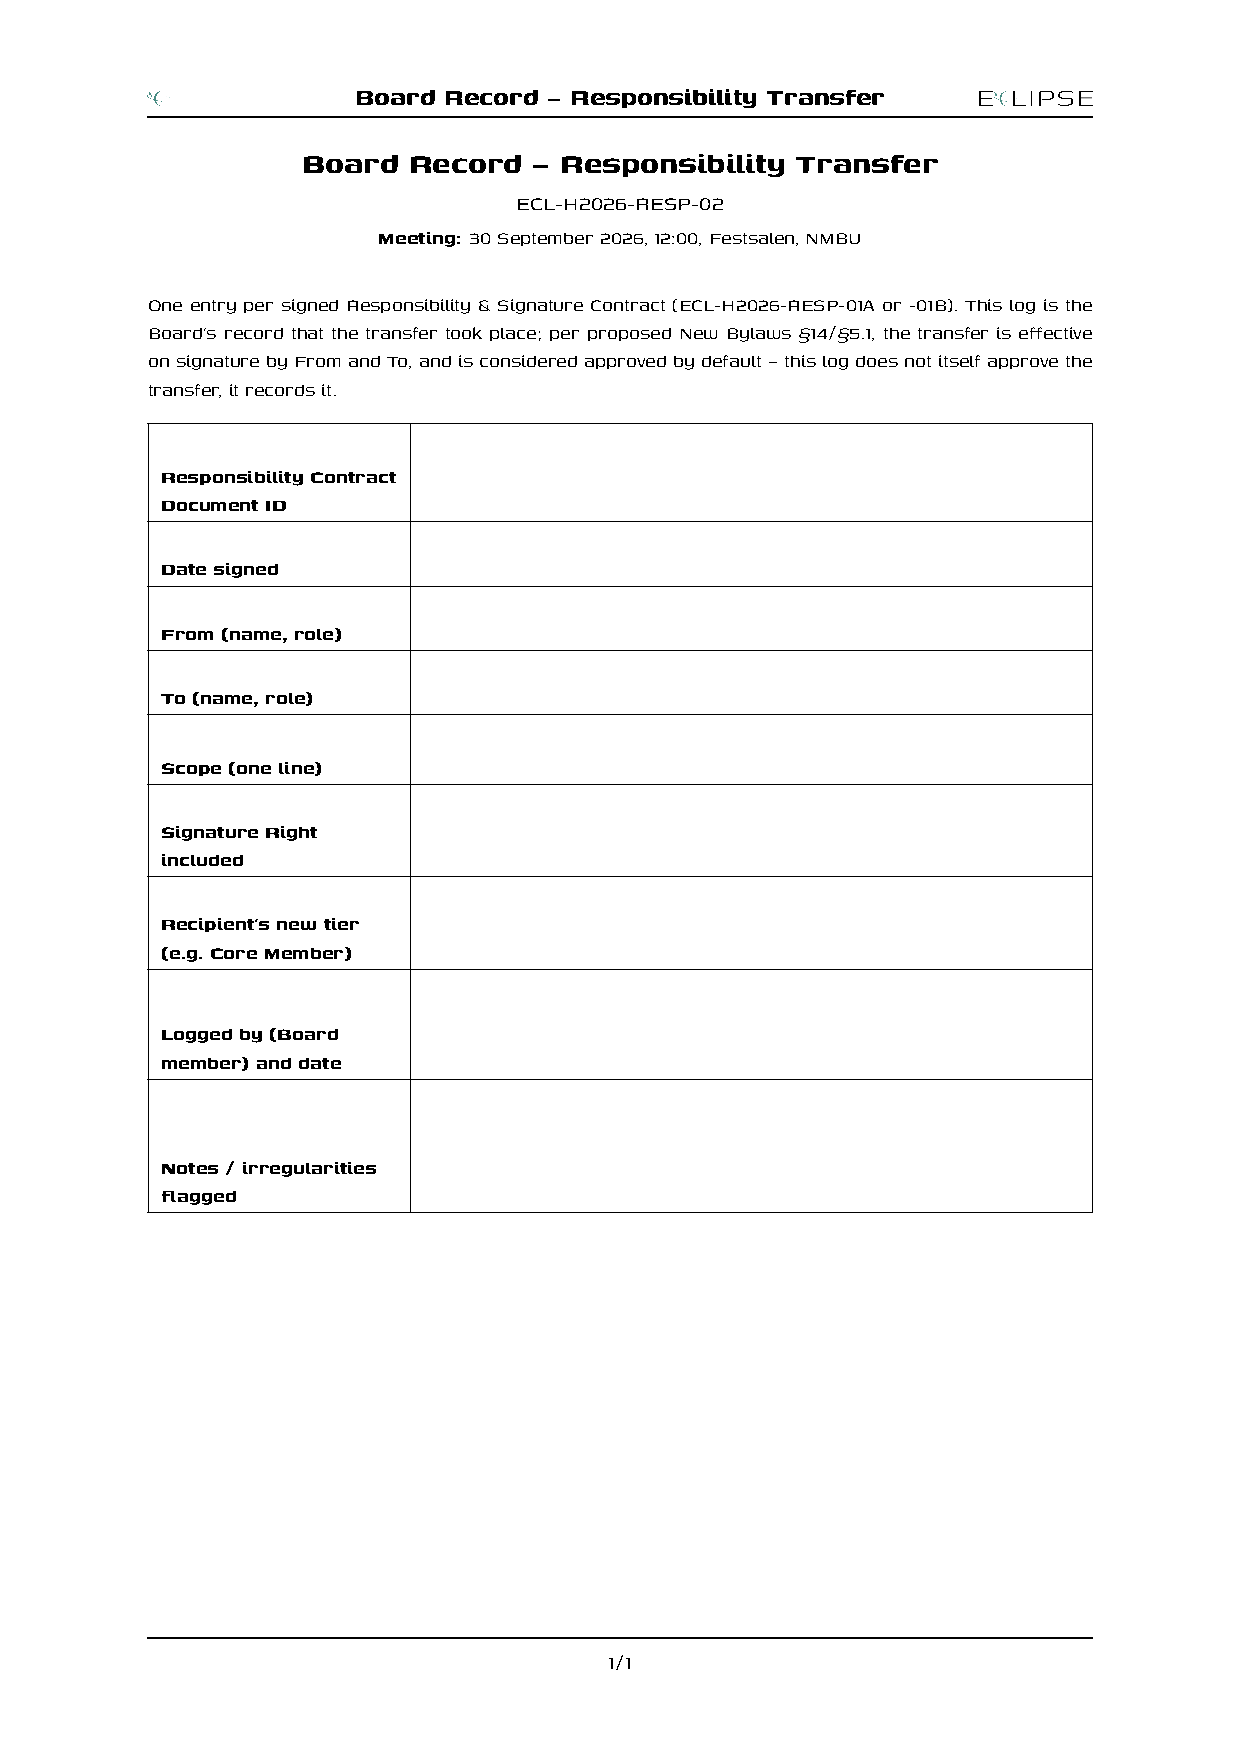
\includepdf[pages=-]{../14 Responsibility and Signature Contract/26H-ECL-GA-RESP2.pdf}

\includepdf[pages=-]{../15 GF for Dummies/26H-ECL-GA-DUMMY1.pdf}

\includepdf[pages=-]{../16 Multilingual Organisational Glossary/26H-ECL-GA-GLOSS1.pdf}

\clearpage
\strut\label{fullcontentend}

% Pad with blank pages so the total page count is a multiple of 8, for
% book-binding in 8-page signatures. \getpagerefnumber reads the page
% number of \label{fullcontentend} as of the previous compile run, so
% this needs two compile passes (handled automatically by latexmk) to
% converge on the correct number of blank pages.
\ExplSyntaxOn
\int_new:N \g_ec_totalpages_int
\int_new:N \g_ec_blanks_int
% The "+1" accounts for the lastpage package's own trailing \clearpage
% (used to compute \pageref{LastPage} for the footer), which always
% appends one further page after whatever this document last shipped.
\int_gset:Nn \g_ec_totalpages_int { \getpagerefnumber{fullcontentend} + 1 }
\int_gset:Nn \g_ec_blanks_int
  { \int_mod:nn { 8 - \int_mod:nn {\g_ec_totalpages_int} {8} } {8} }
\int_step_inline:nn {\g_ec_blanks_int}
  { \clearpage\thispagestyle{empty}\strut }
\ExplSyntaxOff

\end{document}
